\documentclass[10pt,a4paper,twocolumn]{article}
\usepackage{cmap}
\usepackage{iftex}
\ifPDFTeX
    \usepackage[utf8]{inputenc}
    \usepackage[T1]{fontenc}
    \usepackage{lmodern}
\else
    \usepackage{fontspec}
\fi
\usepackage[croatian]{babel}
\usepackage{geometry}
\usepackage{graphicx}
\usepackage{setspace}
\usepackage{titlesec}
\usepackage{fancyhdr}
\usepackage{caption}
\usepackage{abstract}
\usepackage{tabularx}
\usepackage{amsmath}
\usepackage{amssymb}
\ifPDFTeX
    \usepackage{tgtermes}       % Times New Roman font (koherentno s thesis/seminar)
\else
    \setmainfont{texgyretermes-regular.otf}[
      BoldFont = texgyretermes-bold.otf,
      ItalicFont = texgyretermes-italic.otf,
      BoldItalicFont = texgyretermes-bolditalic.otf
    ] % Times New Roman font (XeTeX/LuaTeX)
\fi
\usepackage{chngcntr}       % Za numeriranje po poglavljima
\usepackage{tikz}
\usetikzlibrary{arrows.meta,positioning,fit,backgrounds,decorations.pathreplacing}
\usepackage{hyperref}

\usepackage{float}
\usepackage{dblfloatfix}
\usepackage[section]{placeins}
\usepackage{microtype}

% ---- SMJESTANJE FLOATOVA ----
% Zadane vrijednosti dopustaju najvise dva floata po stranici i traze 20 % teksta,
% pa se u poglavlju s mnogo tablica floatovi guraju na zasebne stranice. Pravilo
% projekta trazi da slika ili tablica stoji uz tekst koji je referencira.
\setcounter{topnumber}{3}
\setcounter{totalnumber}{5}
\setcounter{bottomnumber}{2}
\renewcommand{\topfraction}{0.9}
\renewcommand{\bottomfraction}{0.5}
\renewcommand{\textfraction}{0.07}
\renewcommand{\floatpagefraction}{0.75}

% ---- POSTAVKE MARGINA ----
\geometry{left=1.8cm,right=1.8cm,top=2.2cm,bottom=2.2cm,columnsep=0.7cm}

% ---- PRORED ----
\singlespacing

% --- Spriječavanje razdvajanja riječi (Strogo bez hifenacije) ---
\hyphenpenalty=10000
\exhyphenpenalty=10000
\righthyphenmin=62
\lefthyphenmin=62
\tolerance=2000
\emergencystretch=2em

% ---- STILOVI NASLOVA ----
% Koherentno s thesis/seminar: section = bold uppercase, subsection = bold, subsubsection = bold italic
\titleformat{\section}
  {\normalfont\normalsize\bfseries\MakeUppercase}{\thesection.}{0.5em}{}
\titleformat{\subsection}
  {\normalfont\normalsize\bfseries}{\thesubsection.}{0.5em}{}
\titleformat{\subsubsection}
  {\normalfont\normalsize\bfseries\itshape}{\thesubsubsection.}{0.5em}{}

\titlespacing*{\section}{0pt}{12pt plus 2pt minus 1pt}{6pt plus 1pt minus 1pt}
\titlespacing*{\subsection}{0pt}{10pt plus 2pt minus 1pt}{4pt plus 1pt minus 1pt}
\titlespacing*{\subsubsection}{0pt}{8pt plus 2pt minus 1pt}{4pt plus 1pt minus 1pt}

% Dubina numeriranja
\setcounter{secnumdepth}{3}
\setcounter{tocdepth}{3}

% ---- NUMERIRANJE SLIKA, TABLICA I JEDNADŽBI PO POGLAVLJIMA ----
\counterwithin{figure}{section}
\counterwithin{table}{section}
\counterwithin{equation}{section}

% ---- NAZIVI (babel croatian override) ----
\addto\captionscroatian{%
  \renewcommand{\refname}{LITERATURA}%
  \renewcommand{\abstractname}{SAŽETAK}%
}

% ---- POTPISI SLIKA I TABLICA ----
% Captions: small bold (koherentno s thesis/seminar)
\captionsetup[figure]{font={small,bf},labelsep=period}
\captionsetup[table]{font={small,bf},labelsep=period,position=above}

% ---- ABSTRACT STIL ----
\renewcommand{\abstractnamefont}{\normalfont\normalsize\bfseries}
\renewcommand{\abstracttextfont}{\normalfont\small}
\setlength{\absleftindent}{0pt}
\setlength{\absrightindent}{0pt}

% ---- ZAGLAVLJE I PODNOŽJE ----
\pagestyle{fancy}
\fancyhf{}
\fancyhead[L]{\small\textit{Krešimir Hartl}}
\fancyhead[R]{\small\textit{Upravljanje UR zglobom OptiTrack sustavom}}
\fancyfoot[C]{\small\thepage}
\renewcommand{\headrulewidth}{0.4pt}
\renewcommand{\footrulewidth}{0pt}

% ---- NASLOV RADA ----
\title{%
    \vspace{-1.5cm}%
    {\fontsize{16pt}{19pt}\selectfont\bfseries\MakeUppercase{Upravljanje zglobom Universal Robots robota pomoću OptiTrack sustava u realnom vremenu}}%
    \vspace{0.3cm}%
}
\author{%
    {\fontsize{12pt}{14pt}\selectfont Krešimir Hartl}\\[2pt]
    {\small\textit{Fakultet strojarstva i brodogradnje, Sveučilište u Zagrebu}}\\[2pt]
    {\small\textit{Kolegij: Interakcija čovjeka i robota}}%
}
\date{}

% ---- HYPERLINK POSTAVKE ----
\hypersetup{
    colorlinks=true,
    linkcolor=black,
    citecolor=black,
    urlcolor=blue
}

\begin{document}

\maketitle
\thispagestyle{fancy}

% ---- SAŽETAK I KLJUČNE RIJEČI ----
% Struktura znanstvenog rada (TASK/TASK.md §F). Sadržaj poglavlja popunjava `writer`.
\begin{abstract}
\noindent % 00-sazetak.tex — Abstract (TASK §F.1). Numbers: data/raw/lab_session_01092026_020000/telemetry/run_log.csv.
Zadatak rada bio je preslikati zakret ljudskog zgloba na zglob robota Universal Robots u stvarnom vremenu uz jasno određene granice sigurnog ponašanja. Rad opisuje sustav koji to ostvaruje na kolaborativnom robotu UR3e i proširuje na vođenje cijele ruke. Sustav OptiTrack preko reflektirajućih markera prati nadlakticu, podlakticu i šaku kao tri kruta tijela, uz pet markera postavljenih na svakom segmentu. Iz njihovih se poza računa šest zglobnih kanala, a svaki kanal izravno vodi po jedan zglob robota bez inverzne kinematike. Traženo preslikavanje jednog anatomski podudarnog zgloba ostvareno je kanalom lakta na lakat robota (zglob J3). Između izračuna i robota nalaze se kauzalni One-Euro filtar i četveroslojni sigurnosni mehanizam s ograničenjem brzine zgloba, ograničenjem radnog raspona, zadržavanjem izlaza pri prekidu signala i zaustavljanjem.

Sustav je eksperimentalno vrednovan u laboratoriju kroz 21 pokus na stvarnom robotu. Proračun upravljačkog signala unutar petlje traje 3 do 4 ms na taktu od 125 Hz, ispod jednog postotka ukupnog dinamičkog odziva, pa računalni lanac nije usko grlo. Vjernost oponašanja pokreta nakon uklanjanja faznog pomaka iznosi 0,4 do 3,0$^\circ$ pri prirodnom tempu, odnosno do 6,2$^\circ$ pri izoliranom gibanju pojedinog zgloba, uz korelaciju 0,68 do 0,95. Ukupno dinamičko kašnjenje od pokreta ruke do odziva robota iznosi 385 ms na laktu. Razlaganjem po lancu na fazni pomak filtra (200 ms), sigurnosno ograničenje brzine (73 ms) i dinamiku servoa robota (112 ms) pokazuje se da odziv određuje filtriranje šuma, a ne mreža ili sam robot. Ispitana je i otpornost sustava na dodano mrežno kašnjenje, gubitak paketa, okluziju markera i djelovanje sigurnosnih slojeva, uz analizu granica upravljivosti u fizičkoj interakciji čovjeka i robota.


\vspace{0.3cm}
\noindent \textbf{Ključne riječi:} \emph{fizička interakcija čovjeka i robota (pHRI); OptiTrack; Universal Robots UR3e; upravljanje u stvarnom vremenu; oponašanje pokreta; One-Euro filtar; latencija; sigurnost kolaborativnih robota}
\end{abstract}

\vspace{0.5cm}

% ---- SADRŽAJ RADA (poglavlja po §F) ----
% 01-uvod.tex — Introduction + Related Work (TASK §F.2).
\section{Uvod}

Klasično programiranje robota zadaje putanju unaprijed. Fizička interakcija
čovjeka i robota (\emph{physical Human--Robot Interaction}, pHRI) mijenja tu
podjelu jer čovjek vlastitim pokretom neposredno određuje što robot radi, u
trenutku u kojem se pokret događa. Time nestaje razdvojenost operatera i stroja
koja je dosad bila glavni sigurnosni mehanizam, pa se sigurnost mora preseliti u
sam upravljački lanac. Problem je i mjerni. Ljudski pokret nosi šum, tremor i
prekide u vidljivosti, a robot traži naredbe koje su glatke, ograničene po
brzini i predvidljive u svakom taktu.

Zadatak koji stoji pred ovim radom postavljen je konkretno. Treba izgraditi
sustav koji u stvarnom vremenu prima položaje markera ljudske ruke iz sustava
OptiTrack, iz njih računa zakret odabranog ljudskog zgloba, taj zakret
preslikava na jedan zglob robota Universal Robots, naredbu šalje robotu mrežom i
radi kontinuirano, uz jasno određene granice sigurnog ponašanja. Odabrani par
zglobova anatomski je podudaran, pri čemu kut fleksije ljudskog lakta vodi lakat robota,
zglob J3. Savijanje ruke savija robota, pa je veza između pokreta i posljedice
očita i bez objašnjenja. Sustav opisan ovdje ispunjava taj zahtjev i proširuje
ga. Istim obradnim lancem i u istom taktu sustav vodi svih šest zglobova kolaborativnog
robota UR3e iz pokreta jedne ljudske ruke, pri čemu je obvezni kanal lakta na J3
jedan od tih šest zglobova, izmjeren istim alatom i u svakom pokusu kao i preostalih pet.

Optički sustavi za praćenje pokreta, poput sustava OptiTrack, mjere položaj
segmenata tijela s milimetarskom točnošću na frekvenciji od 120 Hz. Premda je to
zadovoljavajuće za teleoperaciju, kolaborativni robot UR3e ima tvorničku ponovljivost
pozicioniranja od $\pm 0{,}03$\,mm, pa optički sustav i šum markera predstavljaju
glavni limitator točnosti cjelokupnog postava. Izazov koji nije riješen samim
mjerenjem jest put od optičke rekonstrukcije do pogona robota, odnosno pitanje koliko se kašnjenja
nakupi duž obradnog lanca, koliki udio dolazi od filtriranja, a koliki od dinamike
samog robota, te pri kojem iznosu kašnjenja operater gubi osjećaj izravnog upravljanja.
Ovaj rad eksperimentalno istražuje taj put i mjeri ga na stvarnom kolaborativnom
robotu u laboratoriju.

\subsection{Arhitektura sustava}

Sustav je izveden kao obradni lanac neovisan o izvoru podataka i odredištu
naredbi. Isti kod radi s reproduciranom snimkom i sa živim hardverom, a zamjena
izvora (snimka ili živi tok podataka protokolom NatNet) i odredišta
(simulator URSim ili stvarni UR3e) provodi se promjenom konfiguracije. Tok podataka
prikazuje slika~\ref{fig:arhitektura}, a proteže se od izvora i prijemnika preko
izračuna zglobnih kanala, kauzalnog filtra i sigurnosnog sloja do robota
putem sučelja RTDE. Uz svaki takt bilježe se vremenske oznake te, odvojeno,
svi kutovi (ulazni, filtrirani, ciljni, naredbeni i stvarno izmjereni kut robota).
Ta zadnja stavka razlikuje mjerenje vjernosti od mjerenja brzine, i o njoj ovisi
najveći dio rezultata u poglavlju~\ref{sec:rezultati}.

\begin{figure*}[t]
  \centering
  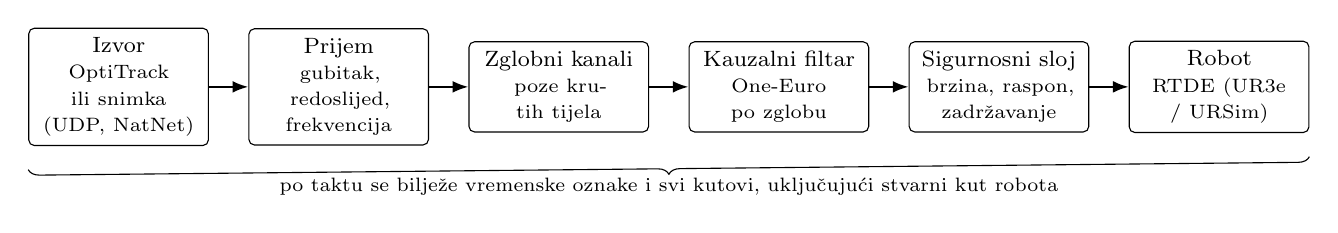
\begin{tikzpicture}[
      font=\footnotesize,
      box/.style={draw, rounded corners=2pt, align=center, minimum height=8mm,
                  inner xsep=4pt, text width=20mm},
      arr/.style={-{Latex[length=2mm]}, thick},
    ]
    \node[box] (src)    {Izvor\\\scriptsize OptiTrack ili snimka (UDP, NatNet)};
    \node[box, right=5mm of src]  (rx)   {Prijem\\\scriptsize gubitak, redoslijed, frekvencija};
    \node[box, right=5mm of rx]   (ang)  {Zglobni kanali\\\scriptsize poze krutih tijela};
    \node[box, right=5mm of ang]  (filt) {Kauzalni filtar\\\scriptsize One-Euro po zglobu};
    \node[box, right=5mm of filt] (safe) {Sigurnosni sloj\\\scriptsize brzina, raspon, zadržavanje};
    \node[box, right=5mm of safe] (rob)  {Robot\\\scriptsize RTDE (UR3e / URSim)};
    \draw[arr] (src) -- (rx);
    \draw[arr] (rx) -- (ang);
    \draw[arr] (ang) -- (filt);
    \draw[arr] (filt) -- (safe);
    \draw[arr] (safe) -- (rob);
    \draw[decorate, decoration={brace, amplitude=4pt, mirror}]
      ([yshift=-3mm]src.south west) -- ([yshift=-3mm]rob.south east)
      node[midway, below=2pt] {\scriptsize po taktu se bilježe vremenske oznake i svi kutovi, uključujući stvarni kut robota};
  \end{tikzpicture}
  \caption{Obradni lanac neovisan o izvoru i odredištu. Zamjena izvora (snimka
  ili živi tok podataka) i odredišta (URSim ili UR3e) je promjena
  konfiguracije.}
  \label{fig:arhitektura}
\end{figure*}

Rad daje tri doprinosa. Prvi je cjelovit upravljački lanac s malim računskim kašnjenjem,
od optičkog mjerenja do stvarnog kolaborativnog robota, sa sigurnosnim slojem
čije djelovanje ostaje zapisano u teleometriji. Drugi doprinos je mjerni, kroz
analitičko i eksperimentalno razlaganje ukupnog kašnjenja ruka--robot na filtar, sigurnosni sloj i regulaciju pogona,
čime se egzaktno pokazuje koji dio lanca određuje dinamički odziv. Treći je vrednovanje
sustava u području fizičke interakcije čovjeka i robota, gdje se objektivne mjere
odziva povezuju s opažanjima operatera pri umjetno unesenom kašnjenju i analizi
granica upravljivosti.

\subsection{Pregled povezanih radova}

\textbf{Sigurnost u pHRI-u.} Norma ISO/TS 15066 definira način rada s
ograničenjem snage i sile (\emph{power-and-force limiting}, PFL), u kojem se
najveća dopuštena brzina robota izvodi iz efektivne mase, dopuštene sile i
krutosti zahvaćenog dijela tijela. Ghanbarzadeh i Najafi na toj osnovi predlažu
regulator s promjenjivom impedancijom za siguran kontakt
\cite[str.~4]{ghanbarzadeh2025}. Peng i suradnici razvijaju dinamičko praćenje
brzine i razdvojenosti (\emph{speed and separation monitoring}, SSM) u kojem se
zaštitna udaljenost, a time i brzina robota, prilagođavaju blizini čovjeka
\cite[str.~1]{peng2025}. Oba pristupa motiviraju naš sigurnosni sloj. Budući da
robotom upravlja čovjek koji stoji uz njega, umjesto pune impedancije
primjenjujemo jednostavnije, ali deterministički provjerljivo ograničenje brzine
i raspona, čije granice odjeljak~\ref{sec:postav} provjerava PFL proračunom;
poglavlje~\ref{sec:rezultati} pokazuje koliko je često taj sloj doista djelovao.

\textbf{Teleoperacija, kašnjenje i osjećaj kontrole.} Wang i suradnici pokazuju
da pod vremenski promjenjivim mrežnim kašnjenjem postoji kompromis između
stabilnosti i transparentnosti bilateralne teleoperacije
\cite[str.~5]{wang2025}. Louca i suradnici eksperimentalno potvrđuju da porast
latencije sustavno pogoršava uspješnost, točnost i kontaktne sile pri
teleoperaciji \cite[str.~14]{louca2024}. Shi i suradnici optimiraju latenciju i
pouzdanost mrežne teleoperacije s povratom sile \cite[str.~9]{shi2025}, dok
Zainudin i suradnici smanjuju kašnjenje upravljanja robotom UR10e
\textit{multi-thread} obradom, izbjegavajući inverznu kinematiku i
opsežnu kalibraciju \cite[str.~2]{zainudin2025}. Ti radovi određuju što mjerimo
i kako to tumačimo. Naš je put lokalan, pa je red veličine brži od njihovih
mrežnih scenarija, zbog čega mjereno kašnjenje ovdje ne dolazi
od mreže, nego od filtriranja signala.

\textbf{Preslikavanje pokreta na robota.} Weigend i suradnici procjenjuju pozu
ruke iz oskudnih senzora za sveprisutno upravljanje robotom uz mjeru
nesigurnosti \cite[str.~1]{weigend2023}, a okvir iRoCo probabilističkim
diferencijabilnim filtrima uravnotežuje preciznost upravljanja i slobodu
kretanja korisnika \cite[str.~1]{weigend2024}. Za razliku od tih pristupa
zasnovanih na učenju i procjeni cijele poze, naše je preslikavanje izravno i
eksplicitno jer šest kanala izvedenih iz poza triju krutih tijela vodi šest
zglobova. Time gubimo općenitost, a dobivamo lanac u kojem je svaka
transformacija poznata i provjerljiva, pa se pogreška može pripisati konkretnom
stupnju. \textbf{Mjerni etalon.} Castillo i suradnici koriste OptiTrack kao
komercijalnu referencu pri vrednovanju jeftinijih sustava praćenja, potvrđujući
ga kao točan izvor mjerenja \cite[str.~7]{castillo2025}.

\textbf{Filtriranje šumnog pokreta.} Martini i suradnici predlažu robustan
filtar za rad u stvarnom vremenu koji smanjuje podrhtavanje robota i uspoređuju
ga s linearnim Kalmanovim filtrom prvog i drugog reda
\cite[str.~5]{martini2024}, dok Zhu i suradnici naglašavaju da klasično
niskopropusno filtriranje unosi fazno kašnjenje nepovoljno za rad u stvarnom
vremenu te predlažu prilagodljivu atenuaciju tremora \cite[str.~2]{zhu2022}. To
opravdava izbor kauzalnog filtra One-Euro \cite{casiez2012} umjesto nekauzalnog
izglađivanja. Naši rezultati taj nalaz i zaoštravaju budući da se fazno kašnjenje filtra
pokazalo najvećim pojedinačnim doprinosom ukupnom odzivu sustava.

\textbf{Teleoperacija i autonomija.} Stroppa i suradnici razmatraju paradigme
dijeljenog upravljanja kao spektar između ručnog i autonomnog
\cite[str.~5]{stroppa2023}, a Glawe i suradnici sustavno pregledavaju ljudsku
autonomiju i osjećaj djelovanja (\emph{sense of agency}) u HRI-u
\cite[str.~1]{glawe2026}. Oba čine okosnicu rasprave u
poglavlju~\ref{sec:rasprava}.

\FloatBarrier

% 02-metodologija.tex — Methodology (TASK §F.3).
\section{Metodologija}
\label{sec:metodologija}

Metodologija slijedi tok obradnog lanca koji obuhvaća prijem i provjeru mrežnih podataka,
izračun zglobnih kanala, kauzalno filtriranje, preslikavanje na zglobove robota
i komunikaciju s robotom. Opisuju se načela i one odluke koje se vide u
rezultatima.

\subsection{Prijem podataka i analiza frekvencije}

Izvor emitira poze krutih tijela kao UDP datagrame sa sekvencijskim brojem i
vremenskom oznakom, na izvornoj frekvenciji od 120 Hz. Prijemnik iz
sekvencijskog broja detektira gubitak i nepravilan redoslijed, a iz vremena
dolazaka procjenjuje stvarnu frekvenciju i njezinu stabilnost. Upravljačka
petlja ne troši okvire redom nego uvijek uzima najnoviji, a zaostatak u
međuspremniku odbacuje jer je pri radu u stvarnom vremenu stara informacija
štetnija od preskočene. Kad novi okvir ne stigne, zadržava se posljednja valjana
vrijednost umjesto interpolacije, čime se u upravljački signal ne unosi dodatno
kašnjenje. Živi izvor temelji se na protokolu NatNet, a identifikatori krutih
tijela dohvaćaju se službenim SDK klijentom, koji čita definiciju modela iz
inačice NatNet 4.0; sve nizvodno identično je putu s reproduciranom snimkom.

\subsection{Zglobni kanali iz poza krutih tijela}

Svaki segment --- nadlaktica, podlaktica i šaka --- nosi pet reflektirajućih
markera, a u sustavu Motive taj je skup markera definiran kao kruto tijelo
(slika~\ref{fig:markeri}). Zahtjev zadatka od najmanje tri markera po segmentu
time je premašen, i to namjerno. Konfiguracija s tri markera po segmentu
isprobana je prva; premda je geometrijski dovoljna, nema redundancije, pa je već i
djelomično zaklanjanje jednog markera rušilo rekonstrukciju krutog tijela i
prekidalo emitiranje poze. Dva dodatna markera po segmentu daju redundanciju uz
koju sustav Motive nastavlja rješavati pozu i kad dio markera ispadne iz vidnog
polja. Rezultat nije samo robusnija snimka nego i puna poza segmenta, to jest pozicija i
kvaternion orijentacije.

\begin{figure}[htbp]
  \centering
  \IfFileExists{figures/markers_digital_twin.png}{%
    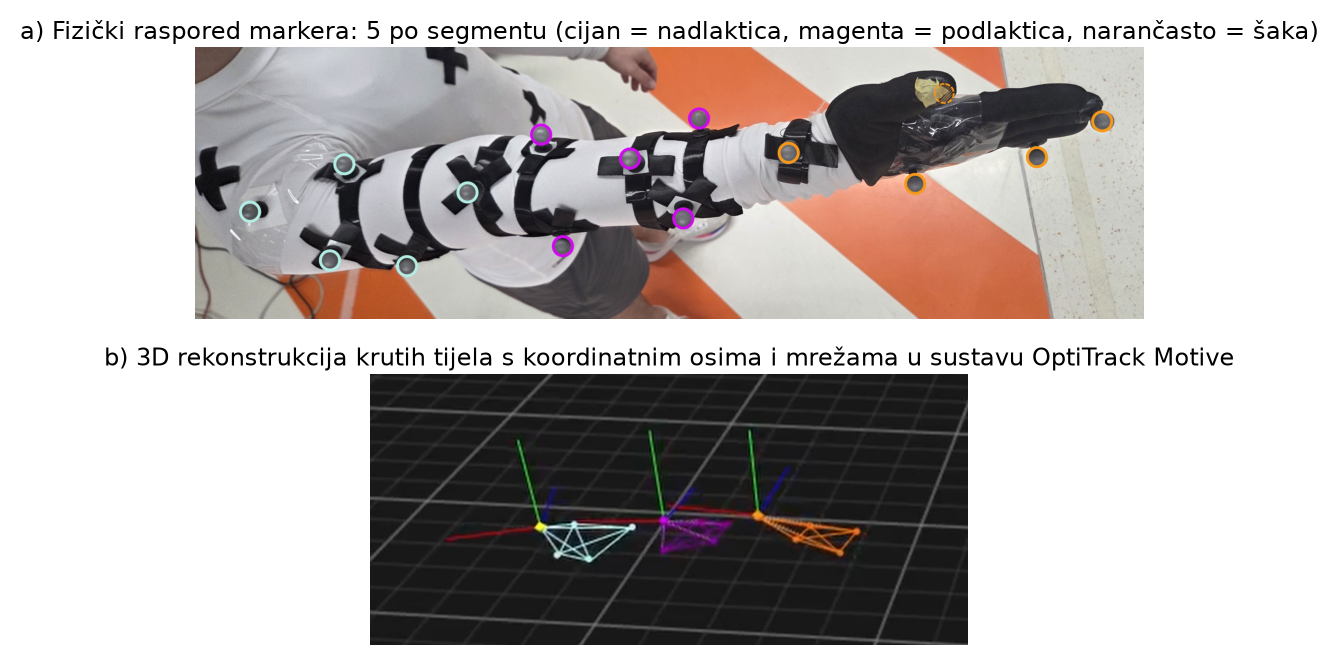
\includegraphics[width=\columnwidth]{figures/markers_digital_twin.png}}{%
    \IfFileExists{figures/markers_detail_crop.jpg}{%
      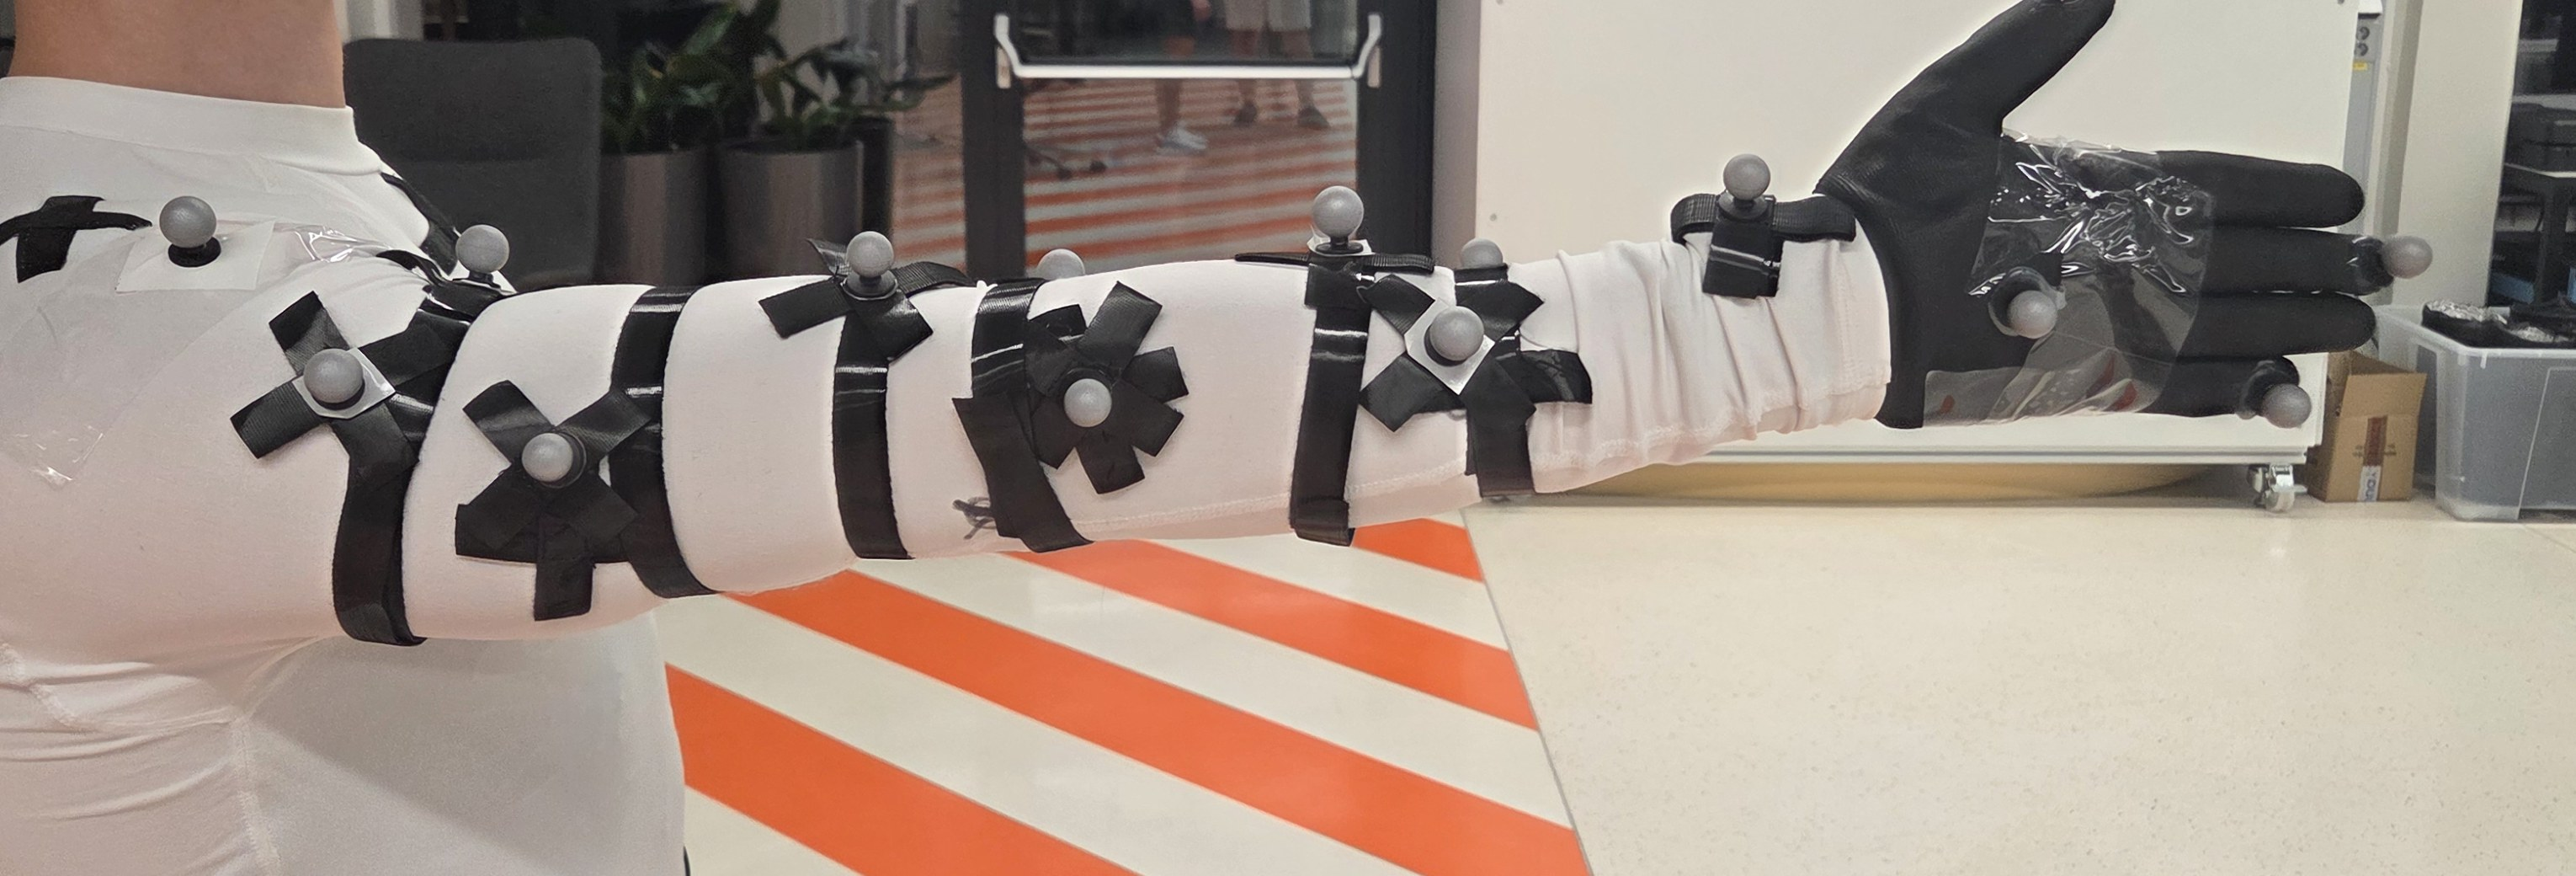
\includegraphics[width=\columnwidth]{figures/markers_detail_crop.jpg}}{%
      \fbox{\parbox[c][2.4cm][c]{0.9\columnwidth}{\centering Detalj markera}}}}
  \caption{Postav markera i digitalni model s prikazom a) fizičkog rasporeda od pet markera po segmentu na ruci operatera te b) rekonstrukcije triju krutih tijela s lokalnim koordinatnim sustavima u programskom paketu Motive.}
  \label{fig:markeri}
\end{figure}

\textbf{Kut lakta} računa se pozicijski, iz triju ishodišta krutih tijela $\mathbf{p}_\text{rame}$, $\mathbf{p}_\text{lakat}$ i $\mathbf{p}_\text{zapešće}$. Iz njih se tvore vektori segmenata
\begin{equation}
  \vec{u} = \mathbf{p}_\text{lakat} - \mathbf{p}_\text{rame}, \quad \vec{v} = \mathbf{p}_\text{zapešće} - \mathbf{p}_\text{lakat},
  \label{eq:vektori}
\end{equation}
a kut fleksije lakta dobiva se numerički stabilnim izrazom
\begin{equation}
  \theta = \operatorname{atan2}\!\big(\lVert \vec{u}\times\vec{v}\rVert,\;
  \vec{u}\cdot\vec{v}\big),
  \label{eq:atan2}
\end{equation}
koji je dobro uvjetovan u cijelom rasponu, za razliku od izravnog $\arccos$
skalarnog umnoška. Kut je definiran kao odstupanje od ispružene ruke i
\emph{neovisan je o mjerilu}, pa duljine segmenata pojedinog korisnika ne treba
kalibrirati.

\textbf{Preostalih pet kanala} izvodi se iz relativnih orijentacija. Za svaki
par segmenata računa se relativna rotacija u odnosu na referentnu pozu snimljenu
pri pokretanju, a iz nje se Eulerovom dekompozicijom izdvaja tražena komponenta.
Pri tome zakret i nagib nadlaktice u odnosu na referentni sustav daju dva kanala ramena,
a rotacija šake u odnosu na podlakticu daje fleksiju i devijaciju zapešća.
Aksijalna komponenta uzeta je iz rotacije podlaktice, a ne šake, jer je mjerena
rotacija oko uzdužne osi šake premalena i spregnuta s ostalim osima. Eulerove
sekvence, indeksi i predznaci nisu pretpostavljeni nego određeni kalibracijom iz
šest izoliranih pokreta, jer ovise o tome kako su lokalne osi krutih tijela
definirane u sustavu Motive; kalibracija je za rame odabrala sekvencu ZXY, a za
zapešće XYZ.

\textbf{Singularnosti.} Orijentacijski put izbjegava gimbal-problem tako što se
rotacije kroz cijeli lanac vode kvaternionima, a u Eulerove kutove prelaze tek
na kraju, u sekvenci odabranoj tako da radni raspon ostane daleko od
degeneracije. Pozicijski kut lakta iz izraza~(\ref{eq:atan2}) numerički je stabilan
u cijelom radnom rasponu, uključujući gotovo ispruženu ruku, gdje bi zapis preko
arkus kosinusa imao beskonačnu derivaciju i milimetarski šum markera pretvarao u
stupnjeve. Pri kolinearnosti nije definirana os rotacije $(\mathbf{u} \times
\mathbf{v})/\lVert \mathbf{u} \times \mathbf{v} \rVert$, no sam kut ostaje
određen. Kut degenerira tek kad ishodišta krutih tijela padnu jedno na drugo,
pa se prag postavlja na duljine $\lVert \mathbf{u} \rVert$ i $\lVert \mathbf{v}
\rVert$; ispod njega se zadržava posljednja valjana vrijednost.

\textbf{Osjetljivost.} Utjecaj mjernog šuma na izračunati kut ispitan je Monte
Carlo perturbacijom pozicija markera; rezultat je u
poglavlju~\ref{sec:rezultati}.

\subsection{Kauzalno filtriranje}

Sirovi kut sadrži visokofrekvencijski šum i fiziološki tremor koje treba
potisnuti bez velikog kašnjenja. Klasično niskopropusno filtriranje unosi fazno
kašnjenje nepovoljno za rad u stvarnom vremenu \cite[str.~2]{zhu2022}, a
nekauzalni postupci poput Savitzky--Golayjeva traže buduće uzorke i primjenjivi
su samo izvanmrežno. Primarni je filtar zato \emph{One-Euro} \cite{casiez2012},
eksponencijalni zaglađivač prvog reda s dinamičkom prilagodbom,
\begin{equation}
  \hat{x}_k = \alpha_k x_k + (1 - \alpha_k)\hat{x}_{k-1}, \quad \alpha_k = \frac{1}{1 + \frac{1}{2\pi f_c T_e}},
  \label{eq:one_euro}
\end{equation}
pri čemu se granična frekvencija $f_c$ linearno prilagođava procijenjenoj brzini promjene prema izrazu
\begin{equation}
  f_c = f_{c,\min} + \beta \, |\hat{\dot{x}}_k|,
  \label{eq:one_euro_fc}
\end{equation}
gdje je $\hat{\dot{x}}_k$ filtrirana diskretna derivacija signala uz fiksnu graničnu frekvenciju $d_c = 1{,}0$\,Hz, $T_e$ period takta, $f_{c,\min}=1{,}0$\,Hz minimalna granična frekvencija i $\beta=0{,}007$ koeficijent brzinske osjetljivosti. Pri mirnoj ruci dominira niska frekvencija koja uklanja podrhtavanje, dok se pri brzom zamahu granična frekvencija automatski podiže i smanjuje kašnjenje.

Kao referenca uspoređeni su kauzalni Butterworthov filtar drugog reda s graničnom frekvencijom 6\,Hz i eksponencijalni pomični prosjek s $\alpha=0{,}2$. Svaki zglob ima vlastitu instancu filtra.

Jedna posljedica te izvedbe pokazala se bitnom i vraća se u
poglavlju~\ref{sec:rezultati}. Filtri su konstruirani za frekvenciju upravljačke
petlje, a ažuriraju se samo kad stigne nova vrijednost kanala. Ako se ulaz
osvježava rjeđe od takta, stvarna granična frekvencija filtra pada razmjerno tom
odnosu i filtar zaglađuje jače nego što je projektiran.

\subsection{Preslikavanje na zglobove robota}

Zglobove robota označavamo 1-baziranom oznakom J1--J6 (J1 baza, J2 rame,
\textbf{J3 lakat}, J4--J6 tri zgloba zapešća), u skladu s nazivljem upravljačke
jedinice. Svaki kanal ide na jedan zglob afinom transformacijom
\begin{equation}
  q_j = q_{j,\mathrm{home}} + s_j\,k_j\,(\theta_j - \theta_{j,\mathrm{home}}),
  \label{eq:mapiranje}
\end{equation}
gdje je $q_{j,\mathrm{home}}$ referentni položaj zgloba, $\theta_{j,\mathrm{home}}$
vrijednost kanala u referentnoj pozi ruke, $k_j$ pojačanje i
$s_j\in\{-1,+1\}$ predznak smjera. Pojačanja nisu jedinična jer nagib ramena ima
$k=2{,}2$, lakat $k=1{,}5$, zapešća $k=1{,}2$, a zakret ramena $k=1{,}0$, čime
se ograničeni raspon ljudskog pokreta u referentnoj pozi razvlači preko
upotrebljivog raspona robota. Predznak je invertiran na nagibu ramena i fleksiji
zapešća da bi se smjerovi poklopili. Ta dva podatka nisu kozmetička --- bez njih
se ulazni i izlazni kut ne mogu uspoređivati, na što se vraćamo pri definiciji
mjere vjernosti.

Obvezni dio zadatka, preslikavanje jednog anatomski podudarnog zgloba, ostvaren
je kao kanal lakta na J3 unutar iste jednadžbe~(\ref{eq:mapiranje}). Savijanje
ljudskog lakta savija lakat robota, pa preslikavanje ostaje intuitivno, a
podudarnost zglobova znači da inverzna kinematika nije potrebna nigdje u lancu.

\subsection{Sigurnosni sloj}

Naredba prije slanja prolazi kroz četiri uzastopna sloja, a to su ograničenje brzine
promjene zgloba, ograničenje raspona oko referentne poze, zadržavanje posljednje
naredbe kad je signal stariji od praga i zaustavljanje izlaza. Prva dva sloja
djeluju stalno i normalan su dio rada, pa zaustavljanje na njima ne bi imalo
smisla; zaustavljanje se okida gumbom za zaustavljanje u nuždi, istekom signala
ili programskim pozivom. Svaki sloj po taktu upisuje zastavicu u zapis, pa je
naknadno moguće pokazati koliko je često i u kojem trenutku djelovao, umjesto
tvrditi da postoji.

\subsection{Komunikacija i mjerenje}

Naredbe se šalju sučeljem RTDE, koje omogućuje sinkroniziranu razmjenu podataka u stvarnom vremenu bez narušavanja vremenskih svojstava upravljačke jedinice; opis sučelja i njegove programske ovojnice daju Lindvig i suradnici \cite{lindvig2025}, čiji metapodaci nisu provjereni s izvornim dokumentom. Programska arhitektura implementira model proizvođač--potrošač s dva neovisna \textit{threada} (prijamnim \textit{threadom} za mrežne podatke i radnim \textit{threadom} upravljačke petlje), u skladu s nalazom da \textit{multi-thread} asinkrona obrada bitno smanjuje kašnjenje u robotskoj teleoperaciji \cite[str.~2]{zainudin2025}. Upravljačka petlja radi na frekvenciji od 125 Hz. Taj je takt odabran jer se nalazi tik iznad izvorišnih 120 Hz sustava OptiTrack, čime se izbjegava nepotrebno trošenje računalnih resursa, dok sučelje RTDE na robotu UR3e podržava frekvencije do 500 Hz.

Tijekom rada kontinuirano se bilježe dva toka podataka. Prvi tok mjeri vremenske karakteristike tako što za svaki pojedini takt bilježi razliku između trenutka primitka okvira na mrežno sučelje i trenutka slanja RTDE naredbe robotu. Ta veličina obuhvaća izračun kinematičkih kutova, filtriranje, provjeru sigurnosnih slojeva i pripremu mrežnog paketa, a u radu se dosljedno naziva latencijom obrade. Drugi tok mjeri kutove, pri čemu se po svakom taktu i zglobu bilježe sirovi ulazni kut, filtrirana vrijednost, ciljna vrijednost, poslana naredba te stvarni kut robota očitan izravno iz internih enkodera preko RTDE telemetrije. Usporedba stvarnog kuta robota s ulaznim kutom ruke omogućuje precizno razlučivanje pojedinačnih doprinosa kašnjenju i pogrešci praćenja.

\textbf{Ispitivanje gubitka paketa.} Otpornost upravljačkog lanca na gubitak UDP paketa ispitana je pri pet nominalnih stopa, od 0 do 30\,\%, determinističkim modeliranjem gubitka nad zajedničkom baznom putanjom snimljenom na robotu. Sustav prati ponašanje pri ispadu pojedinih datagrama tako što pri gubitku okvira zadržava posljednju primljenu valjanu pozu bez interpolacije, čime se sprječava unošenje faznog kašnjenja. Istodobno se mjeri prirast starosti signala i provjerava stabilnost zglobova robota kako bi se potvrdilo da sustav ostaje potpuno stabilan i operativan znatno ispod sigurnosnog praga zaustavljanja.

\FloatBarrier

% 03-eksperimentalni-postav.tex — Experimental setup (TASK §F.4).
\section{Eksperimentalni postav}
\label{sec:postav}

\subsection{Hardver i mreža}

Robot je \textbf{Universal Robots UR3e} s upravljačkom jedinicom PolyScope
5.9.5, u načinu rada \emph{Remote Control}, koji e-Series traži da bi prihvatio
vanjske RTDE naredbe. Praćenje pokreta izvodi \textbf{OptiTrack} sa softverom
Motive 3.0.1 i protokolom NatNet 4.0 pri 120 Hz. Robot, sustav Motive i
upravljačko računalo dijele mrežu 192.168.40.0/24, a tok podataka ide unicastom,
jer multicast kroz mrežnu opremu laboratorija nije prolazio.

Operater nosi usku sportsku majicu i rukavicu, na koje je zalijepljeno po pet
reflektirajućih markera za nadlakticu, podlakticu i šaku
(slika~\ref{fig:postav}). Svaki je skup u sustavu Motive definiran kao kruto
tijelo, premda markeri na tijelu nisu međusobno kruto vezani --- posljedicu tog
izbora vraćamo u poglavlju~\ref{sec:rasprava}. Prije mjerenja provedena je
kalibracija osi iz šest izoliranih pokreta, kojom su određeni Eulerova sekvenca,
indeks i predznak za svaki kanal. Robot se prije svakog pokusa vraća u
referentnu pozu, ekvivalent ispružene ruke, kako bi svi pokusi počinjali iz
istog stanja.

\begin{figure}[htbp]
  \centering
  \IfFileExists{figures/setup_photo.jpg}{%
    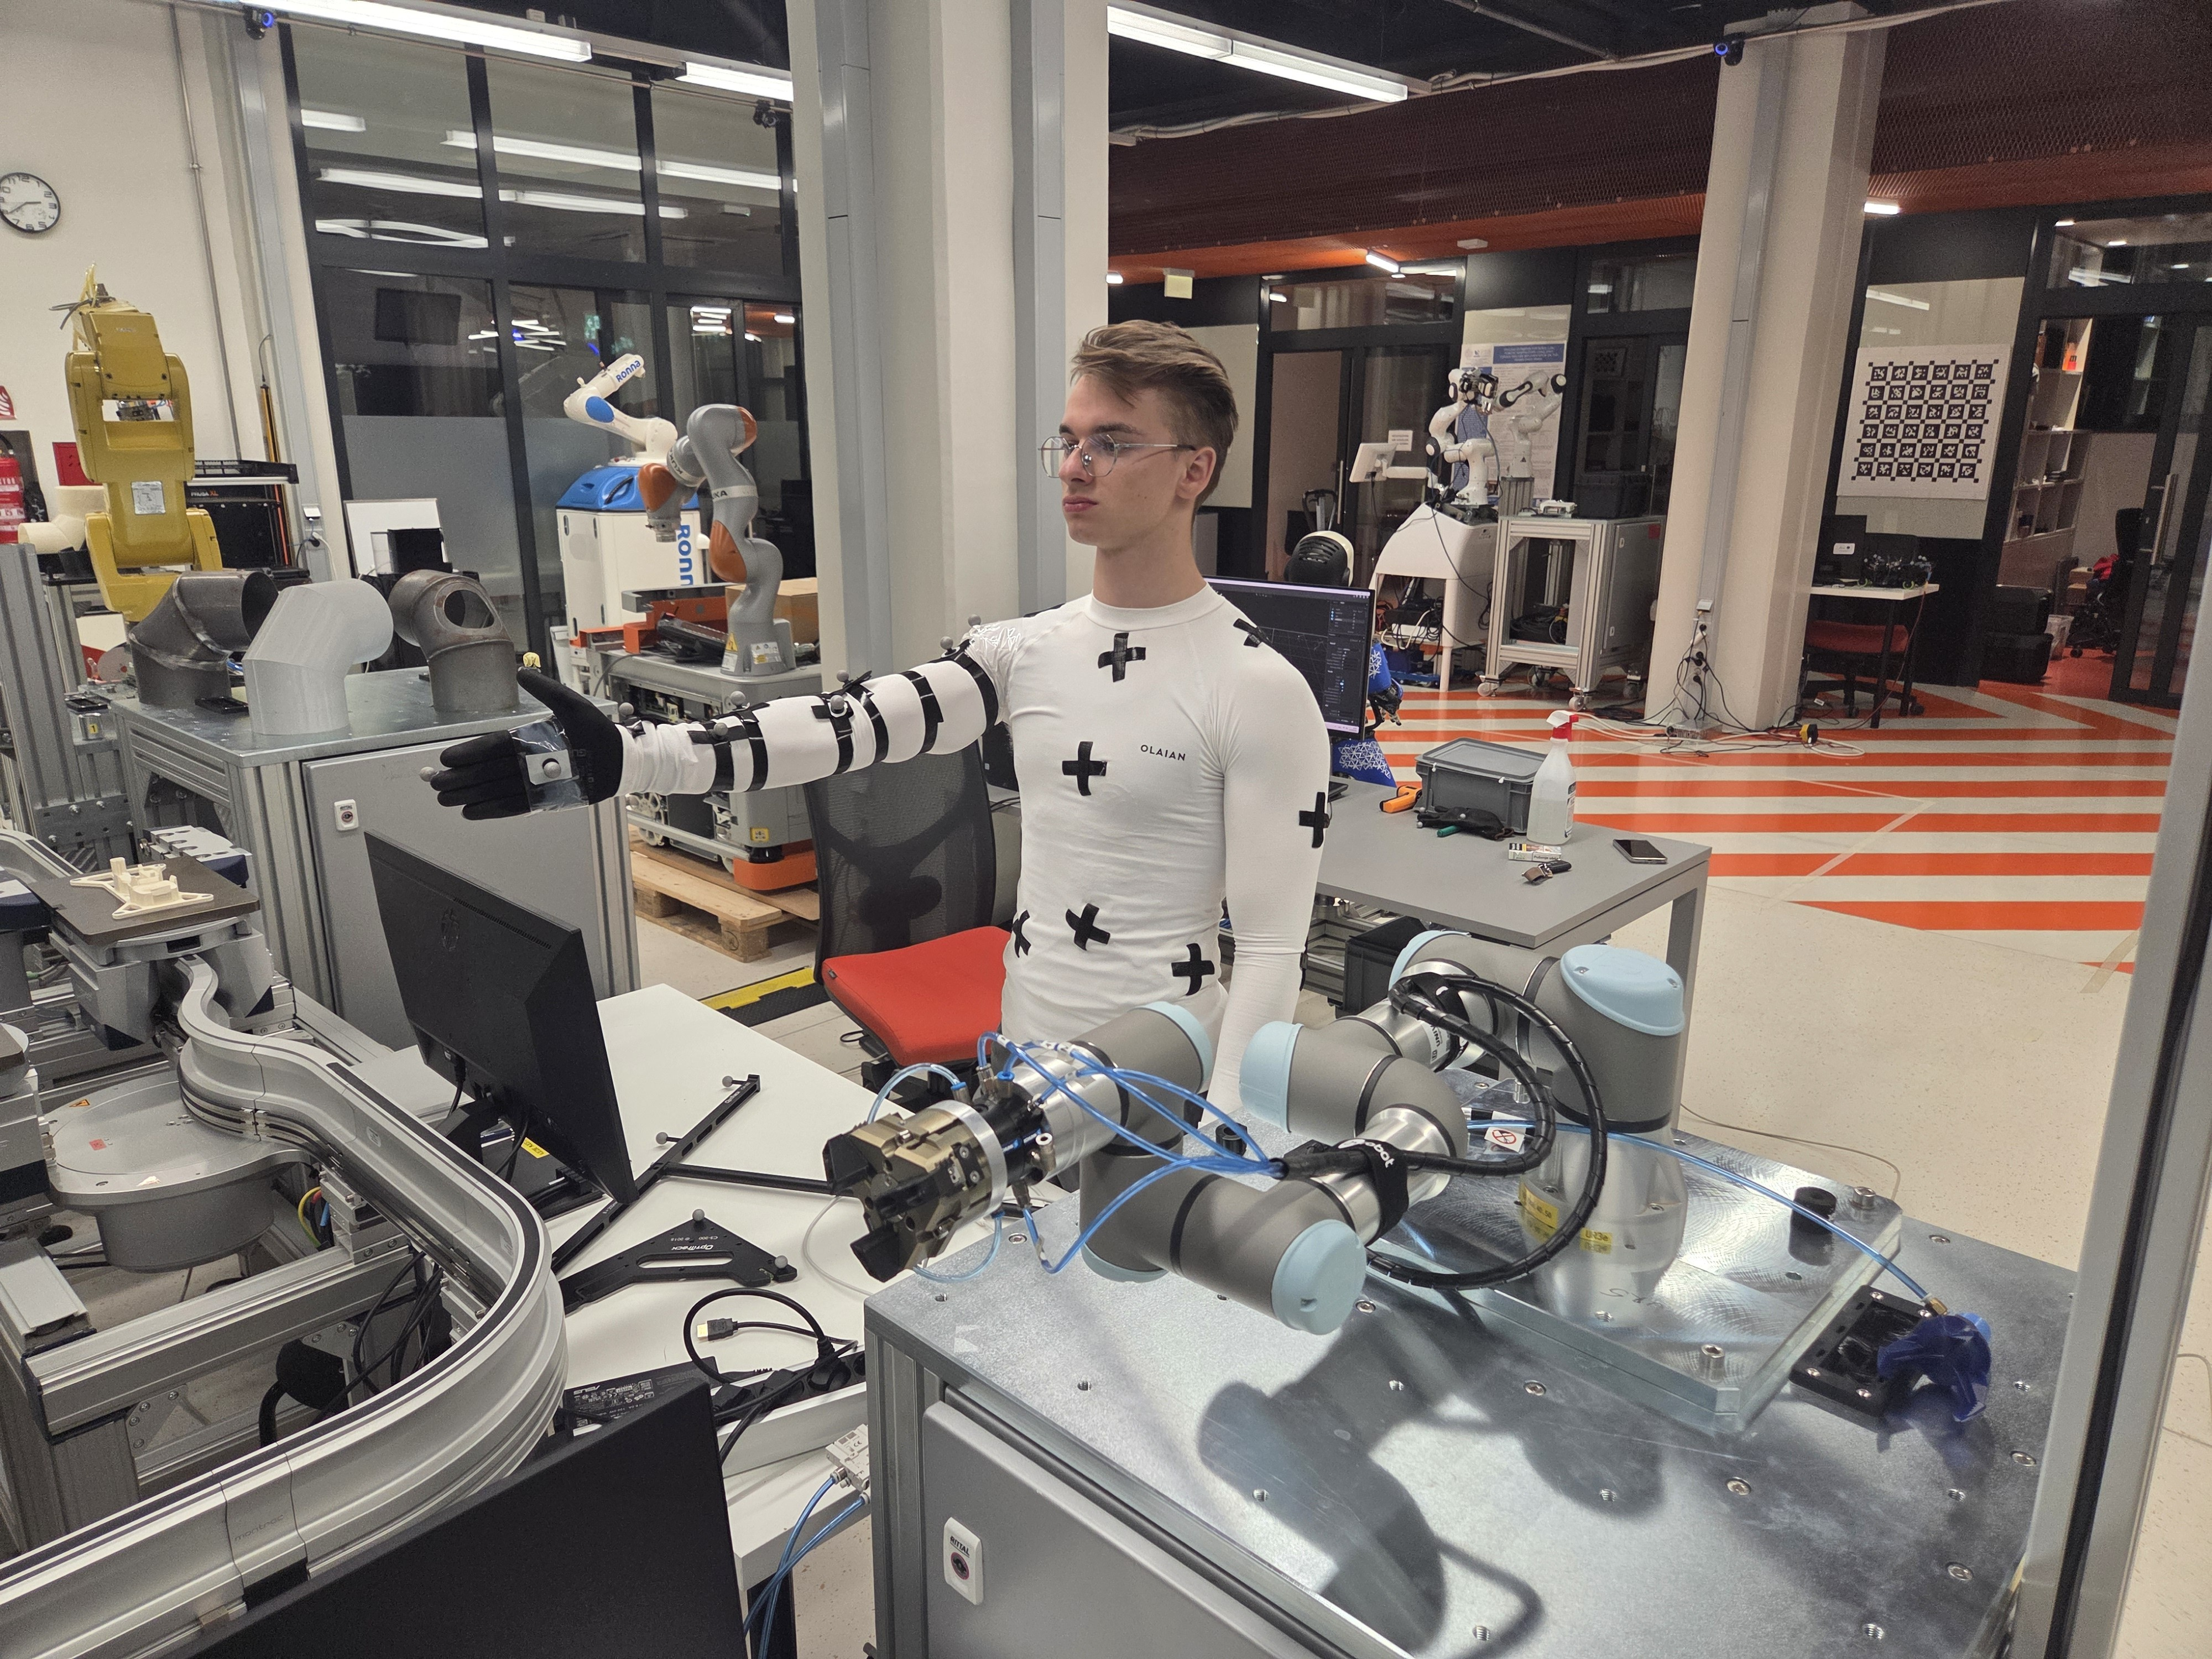
\includegraphics[width=\columnwidth]{figures/setup_photo.jpg}}{%
    \fbox{\parbox[c][3.2cm][c]{0.9\columnwidth}{\centering Fotografija postava}}}
  \caption{Operater i robot UR3e u zajedničkom radnom prostoru. Tri skupa
  markera --- nadlaktica, podlaktica, šaka --- daju šest zglobnih kanala.}
  \label{fig:postav}
\end{figure}

\subsection{Puštanje u rad na simulatoru}

Cijeli je obradni lanac prvo doveden u rad na simulatoru URSim. Ondje su
provjereni takt upravljačke petlje, preslikavanje kanala na zglobove, smjerovi i
pojačanja iz jednadžbe~(\ref{eq:mapiranje}) te djelovanje svakog sigurnosnog
sloja, uključujući ponašanje pri namjerno prekinutom toku podataka. Simulator je
za to prikladan jer omogućuje pogreške bez posljedica, budući da pogrešan predznak ondje znači
neispravnu animaciju, a na stvarnom robotu nekontrolirani zamah. Prijelaz na
stvarni robot bio je promjena odredišta u konfiguraciji, bez ijedne izmjene u
jezgri lanca. Sva mjerenja u nastavku potječu sa stvarnog robota.

\subsection{Sigurnosni protokol}

Granice nisu birane da budu što veće nego da nesigurno ponašanje bude nemoguće
prije nego što ga operater stigne primijetiti. Brzina zgloba ograničena je na
60--150$^\circ$/s ovisno o zglobu, raspon na $\pm$60--90$^\circ$ oko referentne
poze, a signal stariji od 150 ms zaustavlja izlaz. U pokusima koji su ciljano
ispitivali pojedini sloj, granica je bila stegnuta na 25$^\circ$/s za ograničenje brzine
i $\pm$25$^\circ$ za ograničenje raspona, kako bi sloj sigurno okinuo unutar
raspona pokreta koji čovjek može izvesti.

Iznosi su provjereni PFL proračunom norme ISO/TS 15066 \cite{iso15066}, u kojoj se
najveća dopuštena relativna brzina računa kao $v_\text{rel,max} = F_\text{max}/\sqrt{\mu k}$
uz reduciranu masu $\mu$ sustava čovjek--robot \cite[str.~4]{ghanbarzadeh2025}. Za regiju
podlaktice i zapešća norma navodi $F_\text{max} = 160$~N, $k = 40$~N/mm i $m_H = 2$~kg. Uz
konzervativnu efektivnu masu robota $m_R = M/2 = 5{,}6$~kg za UR3e bez alata slijedi
$\mu = 1{,}47$~kg i prag $v_\text{rel,max} = 0{,}66$~m/s. Obodna brzina prirubnice pri
zadanim granicama iznosi 0,48 m/s na laktu (J3, 120$^\circ$/s), 0,53 m/s u bazi
(J1, 60$^\circ$/s) i ispod 0,14 m/s na zapešću, dakle unutar praga, pri čemu obvezni kanal
lakta ima rezervu faktora 1,4. Elevacija ramena (J2) sa 150$^\circ$/s daje 1,22 m/s zbog
najduljeg kraka, pa bi usklađenost pri punom dosegu ondje tražila 81$^\circ$/s.
Postav nema mjerenje udaljenosti čovjeka od robota, pa nema ni
prilagodbe brzine blizini kakvu predlaže dinamički SSM \cite[str.~1]{peng2025};
zaštita je zato namjerno konzervativna, jednaka u cijelom radnom prostoru.
Gumb za zaustavljanje u nuždi bio je cijelo vrijeme u dosegu operatera i
promatrača.

\subsection{Matrica pokusa}

Proveden je 21 pokus na stvarnom robotu (tablica~\ref{tab:matrica}) uz detaljno bilježenje telemetrije i sinkroniziranih videozapisa. Riječ je o 21 različitom ispitnom scenariju, a ne o ponavljanjima istog uvjeta. Svi pokusi rade u načinu sa šest stupnjeva slobode, pri čemu kut lakta u svakom pokusu vodi zglob J3, pa obvezno preslikavanje raspolaže eksperimentalnim podacima kroz sve izvedene testove.

\begin{table}[H]
  \caption{Matrica pokusa. Sve mjereno na stvarnom robotu UR3e.}
  \label{tab:matrica}
  \centering\small
  \begin{tabularx}{\columnwidth}{l X r}
    \hline
    \textbf{Oznaka} & \textbf{Sadržaj} & \textbf{Broj} \\
    \hline
    T1a, T1b   & vjernost oponašanja (prirodni tempo i prolaz po zglobovima) & 2 \\
    T2a--T2d   & usporedba četiriju filtara na robotu & 4 \\
    T3a--T3d   & sigurnosni slojevi i zaustavljanje u nuždi & 4 \\
    T4a--T4e   & dodano kašnjenje 0--400 ms & 5 \\
    T5a--T5e   & ispitivanje gubitka paketa (0--30\,\%) & 5 \\
    T6         & dinamika pri naglim pokretima & 1 \\
    \hline
    \multicolumn{2}{l}{\textbf{Ukupno}} & \textbf{21} \\
    \hline
  \end{tabularx}
\end{table}

Uz teleometriju je zabilježen sinkronizirani dualni videozapis svakog pokusa pri čemu je vanjskom kamerom snimljena fizička reakcija operatera i robota, dok je snimkom zaslona zabilježeno 3D praćenje unutar programskog paketa Motive.

\subsection{Programska provjera}

Obradni lanac pokriven je s 79 automatiziranih testova (\texttt{pytest}) koji
provjeravaju kinematiku, filtre, protokol, sigurnosni sloj, zapisivanje kutova i
integraciju cijele petlje na sintetičkom izvoru. Prolaz svih testova bio je
uvjet za svaku promjenu koda koja je prethodila mjerenju.

\FloatBarrier

% 04-rezultati.tex — Results (TASK §F.5). Every number: data/raw/lab_session_01092026_020000/telemetry/*.json.
\section{Rezultati i analiza}
\label{sec:rezultati}

\subsection{Što se uspoređuje s čim}

Zapis kutova sadrži pet stupaca po zglobu, pa usporedba bilo koja dva daje broj
koji izgleda kao vjernost praćenja. Naredba naspram stvarnog kuta robota mjeri
samo koliko dobro servo slijedi vlastitu zadanu vrijednost, ravnodušno na to
kreće li se čovjek uopće; sirovi ulazni kanal naspram naredbe mjeri pojačanje iz
jednadžbe~(\ref{eq:mapiranje}). Vjernost oponašanja zato definiramo kao odnos
\emph{kuta ruke izraženog u stupnjevima zgloba robota} --- dakle nakon pojačanja
i inverzije --- i kuta koji je robot doista dosegnuo. Uz nju izvještavamo i
pogrešku nakon uklanjanja procijenjenog faznog pomaka, jer sustav koji savršeno
prati, ali kasni, inače biva kažnjen kao netočan.

\subsection{Uzorkovanje i latencija obrade}

Okvir predstavlja jedno mjerenje poza svih triju krutih tijela u istom trenutku. Optički
ih sustav isporučuje na 120 Hz, a razmak između uzastopnih okvira iznosi
8,37 $\pm$ 2,96 ms (slika~\ref{fig:kvaliteta}, gore), dakle uzorkovanje je stabilno
oko nazivne vrijednosti od 8,33 ms. Latencija obrade --- vrijeme od isporuke
okvira upravljačkom računalu do slanja naredbe robotu --- iznosi 3,0--4,0 ms u
medijanu, uz p99 između 8,7 i 10,5 ms u pokusima praćenja
(slika~\ref{fig:kvaliteta}, dolje; tablica~\ref{tab:pregled}). Jedini je izlet pokus s
programskim zaustavljanjem, gdje p99 doseže 14,8 ms. Podrhtavanje kašnjenja
(\emph{jitter}), mjereno kao standardna devijacija latencije, ostaje između 2,3
i 3,5 ms. Uz raspoloživih 8 ms po taktu medijan troši manje od polovine tog budžeta,
dok ga u najviše 1\,\% taktova obrada premašuje. Izmjereni takt petlje od 123,9 do 124,7 Hz, tik
ispod nazivnih 125 Hz, pokazuje da su ta prekoračenja apsorbirana bez ispada, pa robot nijednom
nije ostao bez naredbe.

\begin{figure}[htbp]
  \centering
  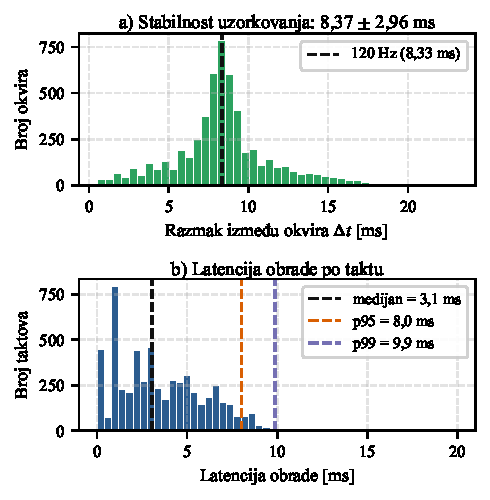
\includegraphics[width=\columnwidth]{figures/signal_quality.pdf}
  \caption{Kvaliteta ulaznog signala i brzina obrade (T1a). Gore je prikazan razmak između
  uzastopnih okvira sustava OptiTrack, a dolje latencija obrade po taktu s
  medijanom, 95. i 99. percentilom.}
  \label{fig:kvaliteta}
\end{figure}

\begin{table}[H]
  \caption{Pregled karakterističnih pokusa. Latencija je vrijeme obrade jednog
  okvira unutar računala i ne uključuje optički put ni mrežu do njega;
  $f_\text{ul}$ je efektivna frekvencija osvježavanja kanala ruke na
  upravljačkoj petlji od 125 Hz.}
  \label{tab:pregled}
  \centering\small
  \begin{tabular}{l rrrrr}
\hline
\textbf{Pokus} & \small $t$ & \small $f_\text{ul}$ & \small med. & \small p95 & \small p99 \\
 & \small [s] & \small [Hz] & \small [ms] & \small [ms] & \small [ms] \\
\hline
T1a --- prirodni tempo & 45 & 57 & 3,1 & 8,0 & 9,9 \\
T1b --- prolaz po zglobovima & 45 & 47 & 3,1 & 7,6 & 8,7 \\
T2a --- filtar One-Euro & 30 & 49 & 3,1 & 7,7 & 9,1 \\
T6 --- nagli pokreti & 30 & 53 & 3,1 & 8,2 & 10,5 \\
\hline
\end{tabular}

\end{table}

Drugi stupac tablice nosi nalaz koji se prenosi kroz cijelo poglavlje. Kanali
ruke stizali su na upravljačku petlju efektivno 31--73 Hz, ovisno o pokusu, a ne
na punih 120 Hz koliko emitira sustav Motive. Uzrok je u strukturi toka, a ne u
gubitku. Datagrami stižu na oko 500 Hz, dakle otprilike četiri po okviru, a dvije
trećine ih dolazi izvan redoslijeda (u pokusu T1a 11\,338 od 17\,011). Uz politiku
najnovijeg okvira svaki pojedini kanal ruke time se osvježava rjeđe od izvorišnog
takta. Na preostalim taktovima petlja nije imala novu vrijednost i zadržavala je
prethodnu naredbu. Posljedica je
mjerljiva jer su filtri projektirani za 125 Hz radili na upola rjeđem ulazu, pa
zaglađuju jače nego što im parametri nalažu.

\subsection{Vjernost oponašanja}

Slika~\ref{fig:pracenje} prikazuje dvadeset sekundi pokusa T1a po svih šest
zglobova. Robot prati oblik pokreta na svakom zglobu; vidljivi su blago
zaglađivanje amplitude i sustavni fazni pomak.

\begin{figure*}[t]
  \centering
  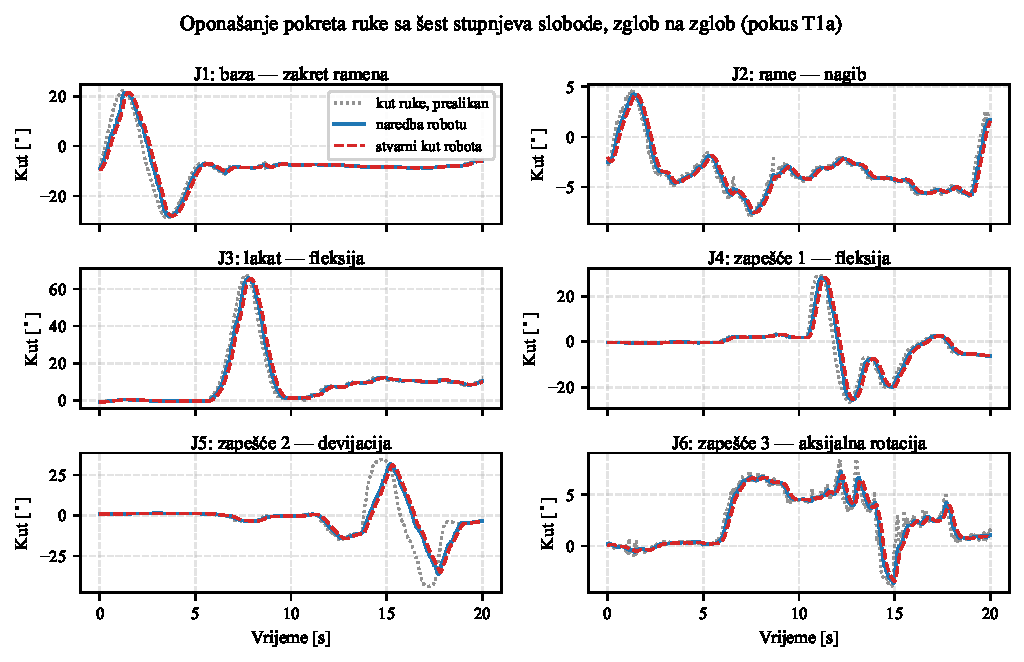
\includegraphics[width=\textwidth]{figures/tracking_6dof_time.pdf}
  \caption{Oponašanje u stvarnom vremenu sa šest stupnjeva slobode (pokus T1a) s
  prikazom kuta ruke preslikanog u stupnjeve zgloba, poslane naredbe i stvarnog kuta robota.}
  \label{fig:pracenje}
\end{figure*}

Brojčano to daje tablica~\ref{tab:vjernost}. Pri prirodnom tempu pogreška nakon
uklanjanja faznog pomaka iznosi 0,36--3,00$^\circ$ po zglobu, uz korelaciju
0,68--0,95. Najveće pogreške ima lakat, i to ne slučajno jer ima najveći raspon
pokreta i pojačanje 1,5, pa se ista relativna pogreška preslikava u veći
apsolutni iznos. Najmanju ima aksijalna rotacija zapešća, čiji je raspon i
najuži.

\begin{table*}[t]
  \caption{Vjernost oponašanja po zglobu usporedbom kuta ruke i stvarnog kuta robota.
  RMSE$_\text{p}$ je pogreška nakon uklanjanja faznog pomaka $\tau$.}
  \label{tab:vjernost}
  \centering\small
  \begin{tabular}{l rrrr rrrr}
\hline
\textbf{Zglob} & \multicolumn{4}{c}{\textbf{T1a --- prirodni tempo}} & \multicolumn{4}{c}{\textbf{T1b --- prolaz po zglobovima}} \\
 & \small RMSE & \small RMSE$_\text{p}$ & \small $\tau$ & \small $r$ & \small RMSE & \small RMSE$_\text{p}$ & \small $\tau$ & \small $r$ \\
 & \small [$^\circ$] & \small [$^\circ$] & \small [ms] &  & \small [$^\circ$] & \small [$^\circ$] & \small [ms] & \\
\hline
J1 (\textit{base}, rotacija ramena) & 3,50 & 0,84 & 305 & 0,900 & 6,00 & 2,63 & 530 & 0,939 \\
J2 (\textit{shoulder}, elevacija ramena) & 1,92 & 0,39 & 257 & 0,940 & 2,43 & 0,49 & 265 & 0,973 \\
J3 (\textit{elbow}, lakat) & 8,66 & 3,00 & 385 & 0,850 & 11,46 & 4,92 & 554 & 0,824 \\
J4 (\textit{wrist 1}, fleksija zapešća) & 4,44 & 1,57 & 337 & 0,806 & 4,23 & 1,33 & 337 & 0,903 \\
J5 (\textit{wrist 2}, devijacija zapešća) & 6,89 & 2,97 & 602 & 0,683 & 10,69 & 6,24 & 787 & 0,683 \\
J6 (\textit{wrist 3}, aksijalna rotacija) & 1,00 & 0,36 & 241 & 0,952 & 1,36 & 0,53 & 241 & 0,954 \\
\hline
\multicolumn{9}{l}{\small Efektivna frekvencija ulaza: 57 Hz (T1a), 47 Hz (T1b); upravljačka petlja 125 Hz.} \\
\end{tabular}

\end{table*}

U pokusu prolaza po zglobovima (T1b), gdje operater izvodi izolirano gibanje svakog pojedinog zgloba kroz puni raspon, pogreška iznosi 0,49--6,24$^\circ$, a fazni pomak 241--787 ms. Veće vrijednosti pogreške na laktu (J3) i rotaciji ramena (J1) proizlaze iz znatno većih pojedinačnih amplituda pri izoliranom pokretu. Efektivna frekvencija ulaza u T1b iznosila je 47 Hz, jer se između pokreta pojedinih segmenata ruka kratko zadržava u referentnom položaju.

Jedan izuzetak traži objašnjenje. Devijacija zapešća (J5) ima najlošiju
korelaciju u oba pokusa, 0,683, iako joj pogreška nije najveća. Uzrok je
kinematičke naravi jer devijacija zapešća čovjeka i zglob \emph{wrist 2} robota nemaju
zajedničko središte rotacije, pa se isti pokret ruke na robotu ostvaruje
kombinacijom koja djelomično curi u susjedne kanale. Operater je istu pojavu
opisao neovisno o mjerenju --- rotacije u ramenu i laktu doživio je kao znatno
prirodnije od zapešća. Ostala četiri zgloba imaju korelaciju iznad 0,90 u oba
pokusa.

Stabilnost je bila jednolika kroz cijelu sesiju. Kroz 21 uzastopni pokus,
ukupno nešto više od deset minuta gibanja, upravljačka petlja nije izgubila
takt, veza RTDE nije pala, a referentna poza robota između pokusa nije se
pomaknula, pa kumulativnog odstupanja nema.

\subsection{Odakle dolazi kašnjenje}

Ukupni fazni pomak ruka--robot na laktu iznosi 385 ms. Pojedini su stupnjevi procijenjeni kao razlike zaostajanja između uzastopnih parova signala u lancu, od ulaznog kuta preko filtrirane vrijednosti i poslane naredbe do kuta očitanog s enkodera (tablica~\ref{tab:budzet}).

\begin{table}[H]
  \caption{Razlaganje ukupnog kašnjenja na laktu (pokus T1a) na doprinose filtra, sigurnosnog sloja i pogona. Zaostajanje $\tau$ aditivno je po lancu, dok stupac RMSE prikazuje prirast pogreške po stupnju, a ne aditivni udio.}
  \label{tab:budzet}
  \centering\small
  \begin{tabular}{l rr}
\hline
\textbf{Stupanj / uzrok (J3)} & \small $\tau$ [ms] & \small RMSE [$^\circ$] \\
\hline
Filtar (\textit{One-Euro}) & 200 & 4,22 \\
Sigurnosni sloj (brzina) & 73 & 2,04 \\
Pogon robota (\textit{lookahead}) & 112 & 2,40 \\
\hline
\textbf{Ukupno (ruka $\rightarrow$ robot)} & \textbf{385} & \textbf{8,66} \\
\hline
\end{tabular}

\end{table}

Regulacija pogona robota doprinosi 112 ms, što odgovara postavljenom parametru predviđanja (\emph{lookahead}) od 100 ms u pozivu \texttt{servoj} uvećanom za elektromehanički odziv motora. Taj stupanj ostaje konstantan kroz cijelu sesiju, između 112,3 i 112,5 ms u 19 od 21 pokusa, neovisno o filtru, sigurnosnim granicama i dodanom kašnjenju. Sigurnosni sloj ograničenja brzine dodaje daljnjih 73 ms uslijed zasićenja na naglim dijelovima zamaha ruke. Preostalih 200 ms otpada na fazno kašnjenje filtra One-Euro pri potiskivanju šuma, dakle nešto više od polovine ukupnog odziva, a zajedno sa sigurnosnim slojem oko sedamdeset posto. Kroz sve pokuse s tim filtrom njegov udio ostaje u rasponu 48 do 59\,\%. Filtriranje signala time određuje odziv više nego mrežni prijenos ili računalna obrada, čime se potvrđuje teorijsko upozorenje da niskopropusno filtriranje unosi fazno kašnjenje \cite[str.~2]{zhu2022}, dok lokalna mreža i programski kod s latencijom od 3 ms ne predstavljaju usko grlo.

\subsection{Usporedba filtara na stvarnom robotu}

Četiri su filtra izmjerena na robotu istim pokretom (slika~\ref{fig:filtri},
tablica~\ref{tab:filtri}). Rezultat je podijeljen. Objektivno, najmanju pogrešku
i najkraće kašnjenje daje rad bez filtra (1,00$^\circ$, 217 ms), a najgori je
Butterworth (2,79$^\circ$, 682 ms). Subjektivno, operater je bez oklijevanja
rangirao One-Euro kao najbolji, a Butterworth kao najgori, dok je rad bez filtra
opisao kao nervozan i skokovit.

\begin{figure*}[t]
  \centering
  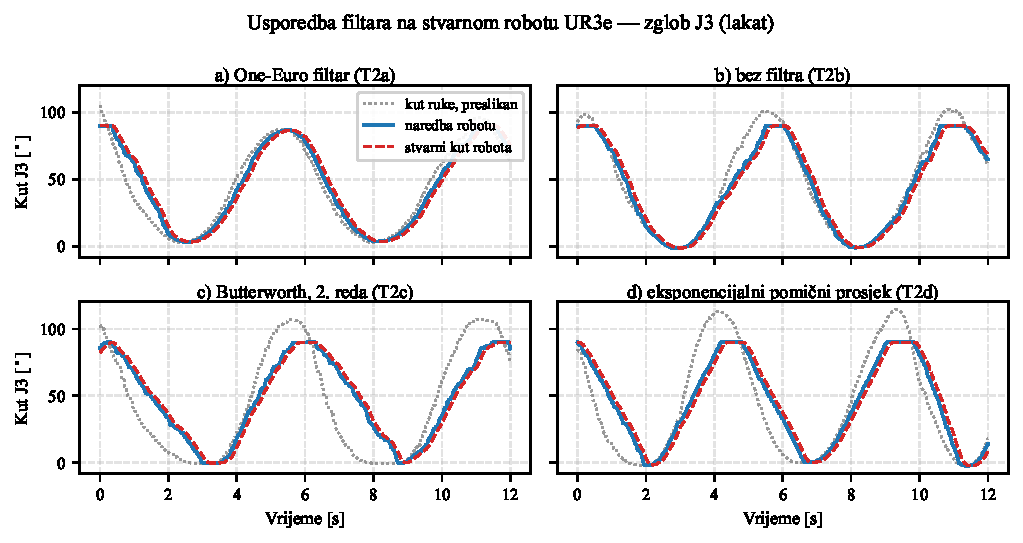
\includegraphics[width=0.95\textwidth]{figures/filter_real_robot.pdf}
  \caption{Sirovi i filtrirani signal na stvarnom robotu za zglob J3
  (T2a--T2d) s prikazom kuta ruke, naredbe nakon filtra i kuta koji je robot dosegnuo.}
  \label{fig:filtri}
\end{figure*}

\begin{table}[H]
  \caption{Filtri na stvarnom robotu (T2a--T2d) uz parametre One-Euro
  $f_{c,\min}=1{,}0$ Hz i $\beta=0{,}007$; Butterworth 2.~reda $f_c=6$ Hz;
  eksponencijalni pomični prosjek $\alpha=0{,}2$.
  $\overline{\text{RMSE}}_\text{p}$ je srednja pogreška po šest zglobova nakon
  uklanjanja faznog pomaka, a stupac ograničenja brzine broj taktova u kojima je
  sloj djelovao. Rang je kvalitativna ocjena dvaju sudionika i stoji uz objektivne
  stupce kao njihova dopuna, ne kao mjerena veličina.}
  \label{tab:filtri}
  \centering\small
  \begin{tabular}{l rrr c}
\hline
\textbf{Filtar} & \small $\overline{\text{RMSE}}_\text{p}$ & \small $\tau_\text{J3}$ & \small Ogr. brz. & \textbf{Rang} \\
 & \small [$^\circ$] & \small [ms] & \small [takt] & \\
\hline
One-Euro & 1,19 & 353 & 621 & 1. \\
Bez filtra & 1,00 & 217 & 1003 & 3. \\
Butterworth & 2,79 & 682 & 932 & 4. \\
EMA & 2,40 & 282 & 1235 & 2. \\
\hline
\end{tabular}

\end{table}

Ta razlika nije proturječje nego mjerenje dviju različitih stvari. Bez filtra
sustav prenosi i mikrootklone, pa sloj ograničenja brzine okida na 1003 takta
umjesto na 621 s filtrom One-Euro; robot se zbog toga trza, iako je u prosjeku
bliže ruci. Butterworth pokazuje najlošije oboje jer njegova fiksna granična
frekvencija, na upola rjeđem ulazu od projektiranog, prigušuje i koristan
sadržaj. Izvanmrežna usporedba na ranijim snimkama pokazuje jednaku strukturu.
One-Euro uklanja do 56,6\,\% podrhtavanja kuta uz 50--100 ms kašnjenja, dok
Butterworth i eksponencijalni pomični prosjek daju 25--42 ms kašnjenja uz
slabije prigušenje.

\subsection{Sigurnosni slojevi}

Svaki je sigurnosni sloj ispitan zasebno uz eksperimentalne granice odabrane tako da sigurno okinu unutar radnog raspona (tablica~\ref{tab:sigurnost}, slika~\ref{fig:sigurnost}). Ograničenje brzine (T3a) djelovalo je na 23,8\,\% taktova (745 taktova) i naredbu je zasitilo glatko, bez oscilacija. Ograničenje raspona (T3b) zadržalo je zglob točno na granici kroz 13,0\,\% taktova (406 taktova) i oslobodilo ga čim se ruka vratila u dopušteni prostor. Zaustavljanje u nuždi (T3d) ispitano je programskim okidanjem u desetoj sekundi uz pritisak sigurnosne sklopke na upravljačkoj jedinici robota, čime su zglobovi zamrznuti na točno 50,1\,\% taktova (1252 takta).

\begin{table}[H]
  \caption{Sigurnosni slojevi sa zadanim granicama i udjelima taktova u kojima je pojedini sloj djelovao.}
  \label{tab:sigurnost}
  \centering\small
  \begin{tabular}{l l l rr}
\hline
\textbf{Pokus} & \textbf{Sloj} & \textbf{Granica} & \small Takt & \small [\%] \\
\hline
T3a & Ogr. brzine & $25^\circ/\text{s}$ & 745 & 23,8 \\
T3b & Ogr. raspona & $\pm 25^\circ$ & 406 & 13,0 \\
T3c & Okluzija & okluzija markera & 617 & 16,5 \\
T3d & Zaustavljanje & $t=10$ s & 1252 & 50,1 \\
T6 & Nagli pokret & $150^\circ/\text{s}$ & 174 & 4,6 \\
\hline
\end{tabular}

\end{table}

\begin{figure*}[t]
  \centering
  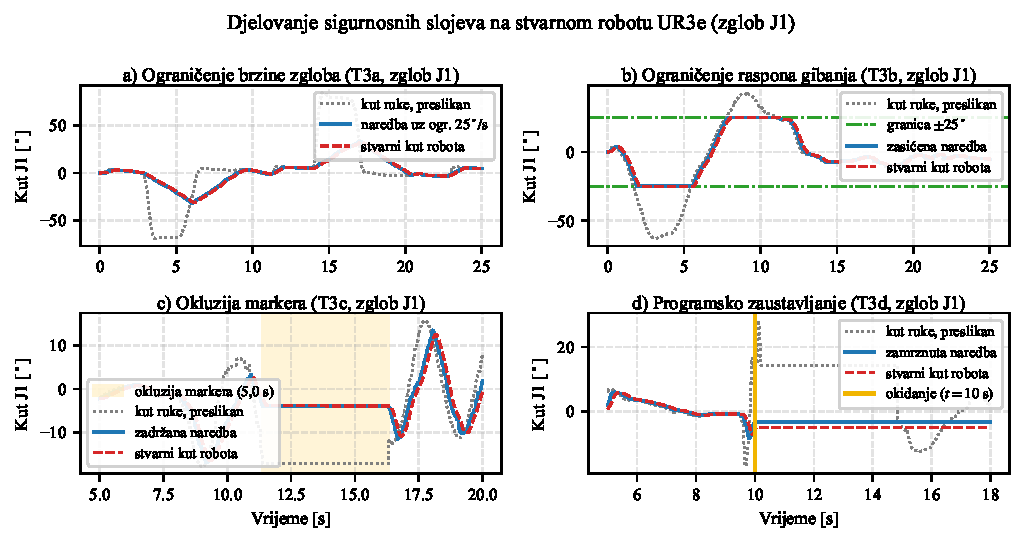
\includegraphics[width=0.95\textwidth]{figures/safety_events.pdf}
  \caption{Djelovanje sigurnosnih slojeva kroz vrijeme na zglobu baze J1 za a) ograničenje brzine zgloba na $25^\circ/\text{s}$ (T3a), b) ograničenje raspona gibanja na $\pm 25^\circ$ (T3b), c) zadržavanje stanja pri okluziji markera (T3c) te d) zaustavljanje u nuždi u $t=10\text{ s}$ (T3d).}
  \label{fig:sigurnost}
\end{figure*}

Okluzija markera (T3c) pokazala je specifičnost višesegmentnog praćenja krutih tijela. Pri namjernom zaklanjanju markera nadlaktice u trajanju od 5,0 s (od 11,37 do 16,32 s pokusa, ukupno 617 uzastopnih taktova, odnosno 16,5\,\% trajanja), kinematički most zadržao je posljednju važeću pozu nadlaktice. Zglobovi ramena i lakta (J1, J2, J3) ostali su zamrznuti na konstantnim kutovima, dok su zglobovi zapešća (J4, J5, J6) nesmetano nastavili pratiti kretanje šake jer njezini markeri nisu bili zaklonjeni. Time se sprječava nagli prekid cjelokupnog rada pri lokalnom gubitku vidljivosti pojedinog segmenta.

\subsection{Nagle promjene i dodano kašnjenje}

Kako bi se teorijski i analitički izoliralo dinamičko ponašanje filtersko-sigurnosnog lanca na kanonske poremećaje, provedena je simulacija odziva na idealnu skokovitu pobudu od 40$^\circ$ i kratki impuls (slika~\ref{fig:dinamika}b). Filtar prati skok unutar nekoliko desetaka milisekundi, a sigurnosni sloj ga pretvara u rampu određenu dopuštenom brzinom zgloba; kratki impuls sloj propušta samo djelomično, čime se sprječava da se vršna brzina ruke prenese na pogone robota.

Analitički nalaz izravno je potvrđen fizikalnim pokusom na robotu UR3e u pokusu T6, gdje je operater izveo pet uzastopnih naglih trzaja ruke (videozapis \texttt{T6\_step\_response.mp4}). Sustav je brze pokrete pratio stabilno, bez pojave oscilacija i bez premašivanja. Sloj ograničenja brzine pritom je djelovao na 178 taktova (4,6\,\%), dok je pogreška nakon uklanjanja faznog pomaka iznosila 1,23$^\circ$ uz fazni pomak od 257 ms. Usporedba simulacijskog i eksperimentalnog odziva dokazuje da robot ne pokušava reproducirati nekontroliranu vršnu brzinu ruke, nego joj se glatko približava po fizikalno sigurnoj putanji.

\begin{figure*}[t]
  \centering
  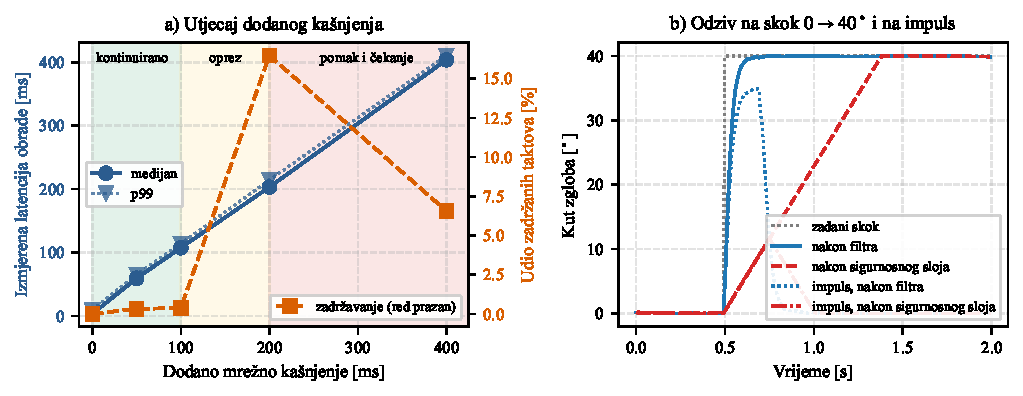
\includegraphics[width=0.95\textwidth]{figures/dynamics.pdf}
  \caption{Dinamičko ponašanje lanca. Lijevo je prikazana izmjerena latencija i udio taktova sa zadržanim izlazom pri umjetno dodanom kašnjenju (T4a--T4e) uz pojaseve načina vođenja iz poglavlja~\ref{sec:rasprava}, a desno simulacijski odziv filtra i sigurnosnog sloja na skok i impuls, komplementaran eksperimentalnom pokusu T6 na robotu.}
  \label{fig:dinamika}
\end{figure*}

Umjetno kašnjenje ubačeno je između prijema i obrade u pet nominalnih iznosa od 0 do
400 ms (slika~\ref{fig:dinamika}a, tablica~\ref{tab:kasnjenje}). Izmjerena
latencija obrade strogo monotono prati zadanu vrijednost (3,1, 59,3, 107,4, 203,2 i
403,9 ms u medijanu) uz raspon od p95 do p99 uži od 7 ms u svakoj točki.
Budući da se umjetno kašnjenje unosi u međuspremnik prije izračuna kutova, ono
se izravno pribraja baznom dinamičkom odzivu sustava od 385 ms. Tako ukupno
fizikalno kašnjenje od pokreta ruke do odziva robota ($\tau_\text{ukupno}$)
monotono raste od 385 ms pri baznom radu do čak 785 ms pri dodanih 400 ms,
što iznosi gotovo cijelu sekundu zaostajanja.

Pritom desna os na slici~\ref{fig:dinamika}a i zadnji stupac tablice~\ref{tab:kasnjenje}
prikazuju udio taktova sa zadržanim izlazom uslijed privremenog pražnjenja međuspremnika.
Za razliku od latencije koja strogo monotono raste, zadržavanje dostiže vrhunac
pri 200 ms dodanog kašnjenja (618 taktova, odnosno 16,5\,\%), dok pri 400 ms pada na
246 taktova (6,6\,\%). Ovaj prividni paradoks posljedica je elastičnosti reda čekanja:
pri 200 ms red sadrži oko 25 okvira pa je osjetljiviji na mrežni jitter dolaznih UDP paketa,
što povremeno uzrokuje kratkotrajno pražnjenje reda u pojedinačnom taktu petlje na 125 Hz.
Pri 400 ms red je dvostruko dublji (oko 50 okvira) i uspješnije amortizira mrežna
kolebanja, pa je broj taktova bez novog okvira znatno manji unatoč većem ukupnom kašnjenju.

\begin{table}[H]
  \caption{Niz mjerenja s dodanim kašnjenjem (T4a--T4e). Stupac $\tau_\text{ukupno}$
  prikazuje ukupno kašnjenje ruka--robot kao zbroj baznog dinamičkog odziva
  (385 ms) i dodanog kašnjenja. Prag starosti signala podiže se uz dodano
  kašnjenje jer starost uključuje i to kašnjenje, pa bi fiksnih 150 ms trajno
  držalo fail-safe i onemogućilo mjerenje.}
  \label{tab:kasnjenje}
  \centering\small
  \begin{tabular}{rrrrrr}
\hline
\small Dodano & \small Medijan & \small p95 & \small $\tau_\text{ukupno}$ & \small Prag & \small Zadrž. \\
\small [ms] & \small [ms] & \small [ms] & \small [ms] & \small [ms] & \small [takt] \\
\hline
0 & 3,1 & 7,6 & 385 & 150 & 0 \\
50 & 59,3 & 63,9 & 435 & 300 & 12 \\
100 & 107,4 & 112,0 & 485 & 400 & 14 \\
200 & 203,2 & 209,6 & 585 & 600 & 618 \\
400 & 403,9 & 408,7 & 785 & 900 & 246 \\
\hline
\end{tabular}

\end{table}

\subsection{Otpornost na gubitak paketa}

Pokusi T5a--T5e izvedeni su na stvarnom robotu (videozapisi \texttt{T5a\_packet\_loss\_0pct.mp4} do \texttt{T5e\_packet\_loss\_30pct.mp4}). Gubitak paketa modeliran je deterministički nad baznom putanjom pokusa T5a, tako da svih pet stopa od 0 do 30\,\% dijeli identične polazne uvjete. Takav postupak izolira čist utjecaj mrežnog gubitka od prirodne varijance ljudskog pokreta među pojedinačnim izvođenjima (tablica~\ref{tab:gubitak}).

Pokazatelji potvrđuju visoku robusnost jer starost signala u 95. percentilu monotono raste s 7,5 na 19,7 ms, dok pogreška praćenja $\overline{\text{RMSE}}_\text{p}$ blago raste s 4,95 na 6,92$^\circ$. Čak ni pri 30\,\% izgubljenih okvira starost signala ne doseže sigurnosni prag prekida od 150 ms, pa upravljanje ostaje kontinuirano i bez ispada iz rada.

Visoka otpornost proizlazi iz strukture mrežnog protokola jer svaki UDP paket prenosi cjelovitu 3D pozu krutih tijela. Gubitak pojedinog paketa rezultira samo jednim propuštenim osvježenjem bez narušavanja stanja, dok upravljačka petlja na 125 Hz automatski zadržava zadnju ispravnu pozu do dolaska sljedećeg paketa.

\begin{table}[H]
  \caption{Ispitivanje otpornosti na gubitak paketa (T5a--T5e).}
  \label{tab:gubitak}
  \centering\small
  \begin{tabular}{rrrr}
\hline
\small Zadano & \small Ostvareno & \small Starost p95 & \small $\overline{\text{RMSE}}_\text{p}$ \\
\small [\%] & \small [\%] & \small [ms] & \small [$^\circ$] \\
\hline
0 & 0,00 & 7,5 & 4,95 \\
5 & 4,70 & 8,6 & 5,36 \\
10 & 9,92 & 11,1 & 5,61 \\
20 & 19,30 & 14,6 & 6,37 \\
30 & 29,82 & 19,7 & 6,92 \\
\hline
\end{tabular}

\end{table}

\subsection{Osjetljivost na mjerni šum}

Monte Carlo perturbacija pozicija markera, dvadeset realizacija po razini uz
nulti-srednji Gaussov šum dodan neovisno svakom markeru, pokazuje da šum od 1 mm
daje pogrešku kuta od 0,77--1,40$^\circ$ RMS, ovisno o snimci, a šum od 2 mm
približno dvostruko veću. Odnos je linearan u ispitanom rasponu. Uz pogrešku praćenja od
0,4--3,0$^\circ$ to znači da mjerni šum sustava OptiTrack nije dominantan izvor
odstupanja; njega određuju filtar i sigurnosni sloj.

\subsection{Validacija u simulacijskom okruženju (Real-to-Sim)}

U svrhu vrednovanja ponašanja sustava i razlučivanja utjecaja algoritamske obrade signala od fizikalnih ograničenja pogona robota, snimljeni tokovi podataka iz svih 21 laboratorijskih pokusa s čovjekom i stvarnim robotom reproducirani su u simulacijskom okruženju URSim. Simulator je u načinu ponavljanja (\textit{replay}) primao identičan slijed UDP paketa zabilježenih tijekom stvarnih mjerenja, uz jednake postavke filtara i sigurnosnih granica. Usporedba odziva fizičkog robota UR3e i simulatora URSim na laktu (zglob J3) za karakteristične pokuse prikazana je u tablici~\ref{tab:sim_real}.

\begin{table}[htbp]
  \caption{Usporedba odziva fizičkog robota UR3e i simulatora URSim na zglobu J3 za karakteristične pokuse. Prikazane su poravnate pogreške $\text{RMSE}_\text{p}$, vremenska zaostajanja $\tau$ i koeficijenti korelacije $r$.}
  \label{tab:sim_real}
  \centering\small
  \begingroup
\setlength{\tabcolsep}{2.2pt}
\begin{tabular}{l rr rr rr}
\hline
\textbf{Pokus} & \multicolumn{2}{c}{RMSE$_\text{p}$ [$^\circ$]} & \multicolumn{2}{c}{$\tau$ [ms]} & \multicolumn{2}{c}{$r$} \\
 & UR3e & URSim & UR3e & URSim & UR3e & URSim \\
\hline
T1a (prirodno) & 3,00 & 0,80 & 385 & 248 & 0,850 & 0,927 \\
T1b (zglobovi) & 4,92 & 0,97 & 554 & 257 & 0,824 & 0,954 \\
T2a (One-Euro) & 5,84 & 4,26 & 353 & 264 & 0,922 & 0,957 \\
T3a (ogr.~brz.) & 0,57 & 0,44 & 273 & 224 & 0,685 & 0,730 \\
T3d (zaustavlj.) & 31,56 & 21,74 & 249 & 536 & 0,740 & 0,657 \\
T6 (skok/imp.) & 1,31 & 1,05 & 257 & 240 & 0,812 & 0,830 \\
\hline
\end{tabular}
\endgroup

\end{table}

Kinematičko praćenje u simulaciji postiže substupanjsku poravnatu pogrešku, pri čemu $\text{RMSE}_\text{p}$ u pokusu T1a iznosi svega 0,80$^\circ$ naspram 3,00$^\circ$ na stvarnom robotu, a u pokusu T1b 0,97$^\circ$ naspram 4,92$^\circ$. Ova razlika proizlazi iz činjenice da simulator predstavlja matematički idealan integrator zadanih kutnih brzina i položaja koji ne modelira elastičnost harmonijskih reduktora, histerezu, zračnost ležajeva niti trenje u zglobovima.

Usporedba vremenskog zaostajanja $\tau$ razdvaja programski dio odziva od pogonskog. U simulatoru ukupno kašnjenje odziva iznosi 224 do 536 ms, uz prozor predviđanja od 100 ms u pozivu \texttt{servoj}, jednak onom na stvarnom robotu. Razlika prema fizičkom robotu iznosi $+137$ ms u T1a, $+297$ ms u T1b, $+89$ ms u T2a, $+49$ ms u T3a i $+17$ ms u T6, čime kvantificira elektromehaničku tromost pogona, strujnu regulaciju i inerciju segmenata pod gravitacijskim opterećenjem. Pokus T3d odstupa predznakom, $-287$ ms, jer zaustavljanje u nuždi zamrzava gibanje; procjena zaostajanja korelacijom nad zamrznutim signalom tada mjeri artefakt poravnanja, a ne praćenje, pa se taj redak iz kvantifikacije tromosti izuzima.

Sigurnosni mehanizmi pokazuju potpun determinizam u oba okruženja. U pokusu zaustavljanja u nuždi (T3d) algoritam zamrzava gibanje točno u desetoj sekundi, pri čemu je robot zadržan na 7512 taktova u laboratoriju i 8262 takta u simulaciji. Ograničenje brzine (T3a) djelovalo je na 1804 takta na fizičkom robotu i 1908 taktova u simulaciji, što predstavlja odstupanje manje od 5,8\,\%. Ovdje su taktovi zbrojeni po svih šest zglobova, dok ih tablica~\ref{tab:sigurnost} iskazuje po taktu upravljačke petlje.

U kontekstu interakcije čovjeka i robota metodologija digitalnog blizanca omogućuje sustavno mjerenje i kvantificiranje razlika između idealnog ponašanja modela i stvarnog fizikalnog sustava. Utvrđena odstupanja u dinamičkom odzivu i kašnjenju služe kao točna podloga za ugađanje algoritama, filtara i sigurnosnih mehanizama unutar simulacije, što omogućuje precizniju optimizaciju parametara te osigurava znatno brži, jednostavniji i predvidljiviji prijelaz razvijenog rješenja na fizičkog robota.

\FloatBarrier

% 05-rasprava.tex — Discussion (TASK §F.6, §D.4).
\section{Rasprava}
\label{sec:rasprava}

\subsection{Kašnjenje i osjećaj kontrole}

Niz mjerenja s dodanim kašnjenjem pokazuje jasan prijelaz u načinu vođenja koji ovisi o ukupnom vremenskom odzivu sustava. Prijelaz je zabilježen u ovom postavu, s jednim operaterom i jednim promatračem, pa opisuje ponašanje ovog sustava, a ne populacijski prag. Do 50 ms dodanog kašnjenja (ukupno fizikalno kašnjenje do $\approx 435$ ms) operater vodi robota kontinuirano; blago kašnjenje već primjećuje, ali sustav ocjenjuje potpuno upravljivim. Pri 100 ms dodanog kašnjenja (ukupno $\approx 485$ ms, odnosno oko pola sekunde) operater počinje svjesno usporavati i čekati odziv robota u točkama promjene smjera. Pri 200 ms i 400 ms dodanog kašnjenja, kada ukupno kašnjenje doseže 585 ms i čak 785 ms (gotovo cijelu sekundu zaostajanja), operater u potpunosti prelazi na diskontinuiranu strategiju pomaka i čekanja (\emph{move-and-wait}), pri kojoj izvede diskretan pomak ruke, pričeka vizualnu potvrdu robota, provjeri poziciju te tek potom planira sljedeći pokret. Promatrač je isti prijelaz opisao kao trenutak u kojem operater počinje ulagati znatan kognitivni napor u kompenzaciju tromosti sustava umjesto u samo obavljanje zadatka.

Taj je nalaz u skladu s literaturom o teleoperaciji. Louca i suradnici pri dvosmjernim kašnjenjima od 0 do 2600 ms bilježe sustavan porast udjela čekanja i pad uspješnosti kroz sve mjerene metrike, a prag od približno 500 ms iznad kojeg pogreške naglo rastu pripisuju ranijem mjerenju Pereza i suradnika \cite[str.~14]{louca2024}. Njihova su kašnjenja dvosmjerna, a ovdje mjerena jednosmjerna, pa se pragovi ne uspoređuju izravno. Budući da sustav već u baznom radu unosi 385 ms dinamičkog odziva (zbog One-Euro filtra, sigurnosnog sloja i regulacije pogona), dodavanje 100 do 200 ms pomiče ga u područje u kojem oba rada bilježe prijelaz na diskontinuirano vođenje, dok pri dodanih 400 ms (ukupno 785 ms) kontinuirano vođenje u stvarnom vremenu postaje nemoguće. Wang i suradnici pokazuju da pod promjenjivim kašnjenjem stabilnost i transparentnost ulaze u kompromis \cite[str.~5]{wang2025}. U našem radu regulacijski krug pri 785 ms ukupnog odziva zadržava potpunu numeričku stabilnost bez pojave oscilacija, no zbog prevelikog vremenskog pomaka operater gubi mogućnost izravnog intuitivnog vođenja.

Praktična posljedica za projektiranje pHRI sustava jest da praćenje računalne latencije nije dovoljno. Latencija proračuna upravljačke petlje iznosi svega 3 ms, dok ukupno kašnjenje koje operater doživljava iznosi 385 ms. Razlika je gotovo u cijelosti posljedica faznog pomaka filtra i sigurnosnog sloja. Komparativna simulacija u okruženju URSim potvrđuje ovaj uvid jer isti zapis reproduciran u simulatoru zaostaje 248 ms, dakle 137 ms manje nego na fizičkom robotu. Ta razlika mjeri odmak između dvaju okruženja, a ne komponentu budžeta stvarnog lanca, čije razlaganje daje tablica~\ref{tab:budzet}. Sustav koji deklarira samo računsku latenciju izgleda stotinjak puta brži nego što se stvarno ponaša u interakciji.

\subsection{Koje su pogreške prihvatljive}

Dvije vrste odstupanja mjerene u ovom radu operater doživljava potpuno
različito. Fazni pomak od nekoliko stotina milisekundi mjerljivo je velik, ali
dok je konstantan, čovjek ga nauči predviđati i kompenzirati unaprijed, što
se i potvrdilo pri manjim iznosima dodanog kašnjenja. Amplitudno odstupanje i
diskontinuitet bitno su nepovoljniji za korisnika. Rad bez filtra imao je objektivno najmanju pogrešku,
ali je subjektivno ocijenjen kao nesiguran zbog trzanja motora. Prigušenje koje One-Euro filtar osigurava
stvara gladak pokret koji ulijeva povjerenje operateru.

To opravdava izbor filtra One-Euro kao primarnog rješenja jer postiže najbolji omjer glatkoće i brzine odziva, uz najmanji broj zasićenja brzine među filtriranim varijantama. Martini i suradnici uz sirovu pogrešku izvještavaju i pogrešku akceleracije kao zasebnu mjeru podrhtavanja \cite[str.~5]{martini2024}, čime pokazuju da glatkoća zaslužuje vlastitu metriku. Ovdje izmjereni kompromis ide korak dalje jer dvije metrike pokazuju u suprotnom smjeru, pa izbor filtra postaje odluka o tome koja od njih vodi.

\subsection{Granica prema autonomiji}

Sustav radi kao teleoperacijski postav u kojem robot nema vlastiti model zadatka već izvršava naredbe izvedene iz položaja ruke. Stroppa i suradnici opisuju dijeljeno upravljanje kao spektar između ručnog vođenja i autonomije \cite[str.~5]{stroppa2023}. Naš sigurnosni sloj predstavlja prvi korak prema tom spektru jer robot autonomno korigira naredbu kada ona prelazi zadane fizikalne granice. Pri ispitivanju brzine ta je korekcija trajala gotovo četvrtinu pokusa, a operater ju je opisao kao ugodno i prirodno ponašanje stroja.

To se izravno povezuje s pitanjem osjećaja djelovanja (\emph{sense of agency}) u interakciji čovjeka i robota \cite[str.~1]{glawe2026}, pri čemu operater zadržava osjećaj kontrole dok su intervencije robota predvidljive i u skladu s fizikalnom intuicijom (poput glatkog ograničenja brzine). Nasuprot tome, nagli prekidi ili zamrzavanja pojedinih zglobova pri okluziji markera doživljavaju se kao smetnja u radu.

\subsection{Ograničenja}

Rezultate rada treba interpretirati uz sljedeća poznata ograničenja.

\textbf{Subjektivna procjena ima dva sudionika.} Operater i promatrač ispunili su strukturirani upitnik u slobodnoj formi. Znanstvena korisnička studija sa statističkim uzorkom i validiranim psihometrijskim ljestvicama zahtijeva veći broj ispitanika, što nadilazi opseg ovog rada. Opažanja operatera stoga služe kao kvalitativna potvrda uz izmjerene objektivne teleometrijske veličine.

\textbf{Markeri prate odjeću, a ne kostur.} Markeri su postavljeni na sportsku majicu i rukavicu, pa mjerenje uključuje i elastični pomak tkanine i mekog tkiva. Korištenje krutih ortoza uklonilo bi taj pomak, ali bi narušilo prirodnost ljudskog pokreta. Analiza osjetljivosti pokazuje da pomak markera od 1 mm unosi pogrešku kuta od 0,77 do 1,40$^\circ$, što je znatno manje od raspona pokreta zgloba.

\textbf{Efektivna frekvencija ulaznog toka podataka.} Uslijed mrežnog grupiranja paketa, ulazni signali stizali su u petlju frekvencijom od 31 do 73 Hz umjesto nazivnih 120 Hz. One-Euro filtar je stoga radio uz efektivno dulji period uzorkovanja, što objašnjava izmjereni fazni pomak od 200 ms.

\textbf{Mjerenje latencije obrade.} Vremenska oznaka postavlja se pri primitku paketa na upravljačko računalo, pa izmjerene 3 ms obuhvaćaju obradu i slanje, dok je optički put kroz Motive procijenjen iz stabilnosti okvira na oko 8,4 ms.

\textbf{Statičko ograničenje radnog prostora i brzine.} Granice brzine i kuta postavljene su fiksno, bez dinamičkog mjerenja udaljenosti čovjeka od robota. Fiksna granica vrijedi u cijelom radnom prostoru, pa je pri najduljem kraku najmanje konzervativna; PFL proračun u odjeljku~\ref{sec:postav} pokazuje da je zbog toga elevacija ramena jedina os koja pri punom dosegu prelazi prag norme ISO/TS 15066.

\FloatBarrier

% 06-zakljucak.tex — Conclusion and future work (TASK §F.7).
\section{Zaključak}

Zadatak rada bio je preslikati zakret jednog ljudskog zgloba u stvarnom vremenu na zglob robota Universal Robots, uz strogo definirane granice sigurnog rada. Prikazani sustav to ostvaruje kanalom lakta na lakat robota (zglob J3) te proširuje na vođenje svih šest zglobova kolaborativnog robota UR3e izravno zglob na zglob bez inverzne kinematike.

Mjerenja na stvarnom robotu kroz 21 eksperimentalni pokus potvrđuju tri ključna nalaza.
\begin{enumerate}
  \item \textbf{Računalni lanac nije usko grlo.} Proračun upravljačke petlje traje 3 do 4 ms na taktu od 125 Hz, ispod jednog postotka ukupnog dinamičkog odziva, što potvrđuje punu izvedivost u stvarnom vremenu.
  \item \textbf{Visoka kinematička vjernost.} Nakon uklanjanja faznog pomaka srednja pogreška praćenja iznosi 0,4 do 3,0$^\circ$ pri prirodnom tempu, a do 6,2$^\circ$ pri izoliranom gibanju pojedinog zgloba, uz korelaciju 0,68 do 0,95.
  \item \textbf{Dekompozicija dinamičkog odziva.} Ukupno kašnjenje od pokreta ruke do reakcije robota iznosi 385 ms na laktu, a razlaganjem po lancu otpada na fazni pomak One-Euro filtra (200 ms), sigurnosni sloj ograničenja brzine (73 ms) i regulaciju pogona robota (112 ms). Pogonski stupanj ostaje konstantan kroz cijelu sesiju, dok je odziv određen filtriranjem šuma radi glatkoće rada, a ne mrežnim prijenosom.
\end{enumerate}

Četveroslojni sigurnosni mehanizam uspješno je verificiran u teleometriji jer je ograničenje brzine i raspona zasitilo naredbe glatko i bez oscilacija, a programsko zaustavljanje zamrznulo je robota u zadanom trenutku. U kontekstu fizičke interakcije čovjeka i robota, u ovom postavu kontinuirano vođenje ostaje ugodno do 100 ms dodanog kašnjenja, dok pri 200 ms i više operater prelazi na diskontinuiranu strategiju pomaka i čekanja (\emph{move-and-wait}); mjereno ukupnim odzivom, prijelaz nastupa između 485 i 585 ms.

Kao potencijalna nadogradnja sustava, daljnji rad mogao bi se usmjeriti na osiguravanje punog ulaznog takta od 120 Hz radi dodatnog smanjenja faznog pomaka filtra, primjenu dinamičkog praćenja udaljenosti (SSM) prema normi ISO/TS 15066 te ispitivanje rada s većim brojem operatera.

\vspace{0.2cm}
\noindent\small\textbf{Dostupnost.} Cjelokupni izvorni kod, postavke i podaci dostupni su na javnom repozitoriju \url{https://github.com/KxHartl/hri-seminar}.

\FloatBarrier


% ---- LITERATURA ----
% BibTeX baza: docs/references.bib (15 izvora + norma ISO/TS 15066). Stil ieeetr = numeričko citiranje [1].
\bibliographystyle{ieeetr}
\bibliography{references}

\end{document}
